% Copyright (c) 2010 Jérémie DECOCK (http://www.jdhp.org)

%\documentclass[pdftex,a4paper,11pt]{article} 
\documentclass[pdftex,a4paper,11pt]{report} 
\usepackage[utf8]{inputenc}
\usepackage[frenchb]{babel}
\usepackage[pdftex]{graphicx}
\usepackage{amsmath}
\usepackage{amssymb}
\usepackage{subfigure}
\usepackage{hyperref}

\hypersetup{
	pdftoolbar=true,                    % show Acrobat’s toolbar ?
	pdfmenubar=true,                    % show Acrobat’s menu ?
	pdffitwindow=true,                  % page fit to window when opened
	pdftitle={Pyarm},                   % title
	pdfauthor={Jérémie DECOCK},         % author
	pdfsubject={Pyarm},                 % subject of the document
	pdfnewwindow=true,                  % links in new window
	pdfkeywords={Pyarm},                % list of keywords
	colorlinks=true,                    % false: boxed links; true: colored links
	linkcolor=black,                    % color of internal links
	citecolor=black,                    % color of links to bibliography
	filecolor=black,                    % color of file links
	urlcolor=black                      % color of external links
}

%\newcommand{\reels}{\mathbb{R}}
\newcommand{\vs}[1]{\boldsymbol{#1}} % vector symbol (\boldsymbol, \textbf or \vec)
\newcommand{\ms}[1]{\boldsymbol{#1}} % matrix symbol (\boldsymbol, \textbf)

\numberwithin{equation}{subsection}

\begin{document}

\title{Pyarm}
\author{
	Jérémie \bsc{Decock}
}
\date{\today{}}

\maketitle

%%%%%%%%%%%%%%%%%%%%%%%%%%%%%%%%%%%%%%%%%%%%%%%%%%%%%%%%%%%%%%%%%%%%%%%%%%%%%%%%

\tableofcontents

%%%%%%%%%%%%%%%%%%%%%%%%%%%%%%%%%%%%%%%%%%%%%%%%%%%%%%%%%%%%%%%%%%%%%%%%%%%%%%%%

\chapter*{Introduction}

\dots

%%%%%%%%%%%%%%%%%%%%%%%%%%%%%%%%%%%%%%%%%%%%%%%%%%%%%%%%%%%%%%%%%%%%%%%%%%%%%%%%

\chapter{Modèles de muscles et modèles de bras}

\section{Présentation des modèles}

\subsection{Présentation}

\begin{center}
        \includegraphics[width=.90\linewidth]{fig/muscle4c}
\end{center}

\begin{itemize}
    \item Bras 2D
    \item Plan transverse (Mitrovic, Weiwei) ou sagittal (Kambara)
    \item 2 membres (le bras et l'avant-bras) % ou arrière-bras ou bras supérieur
    \item 2 articulations (épaule et coude)
    \item 6 muscles~:
    \begin{enumerate}
        \item fléchisseur de l'épaule
        \item extenseur de l'épaule
        \item fléchisseur du coude
        \item extenseur du coude
        \item double fléchisseur
        \item double extenseur
    \end{enumerate}
\end{itemize}

Remarque~: la numérotation des muscles est différente dans le modèle de Weiwei.

\subsection{Les modèles étudiés}
Trois modèles ont été étudiés~:
\begin{itemize}
    \item Katayama / Mitrovic \cite{katayama1993, ozkaya1999, mitrovic10, mitrovic2008, mitrovic2009}
    \item Kambara \cite{kambara2009, ozkaya1999}
    \item Brown / Weiwei \cite{brown1999, li2006, li2004, todorov2005}
\end{itemize}

\subsection{Historique}

\begin{center}
        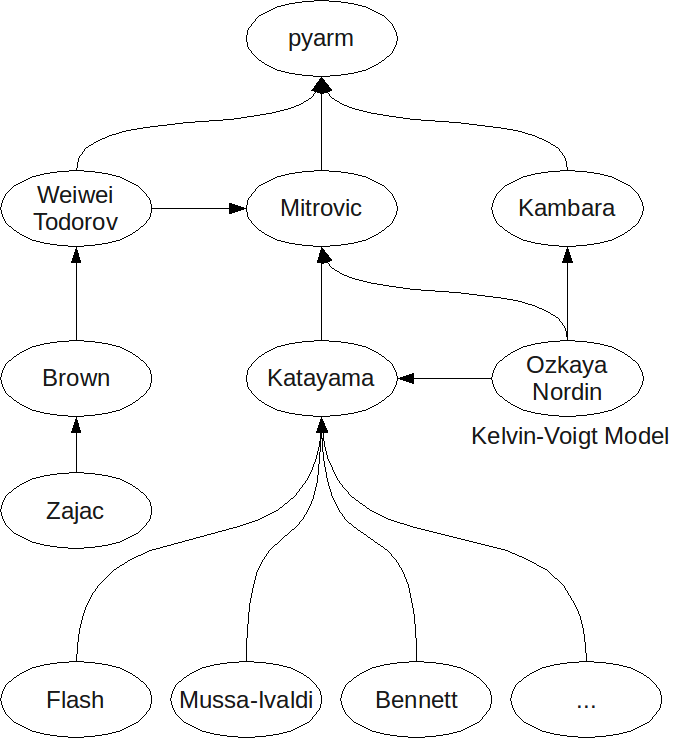
\includegraphics[width=.80\linewidth]{bib}
\end{center}

\subsection{Simulateur Pyarm}

\begin{itemize}
    \item Codé en Python
    \item Implémente les 3 modèles
    \item \url{http://code.google.com/p/pyarm/}
\end{itemize}

%\begin{figure}
%    \centering
%    \subfigure{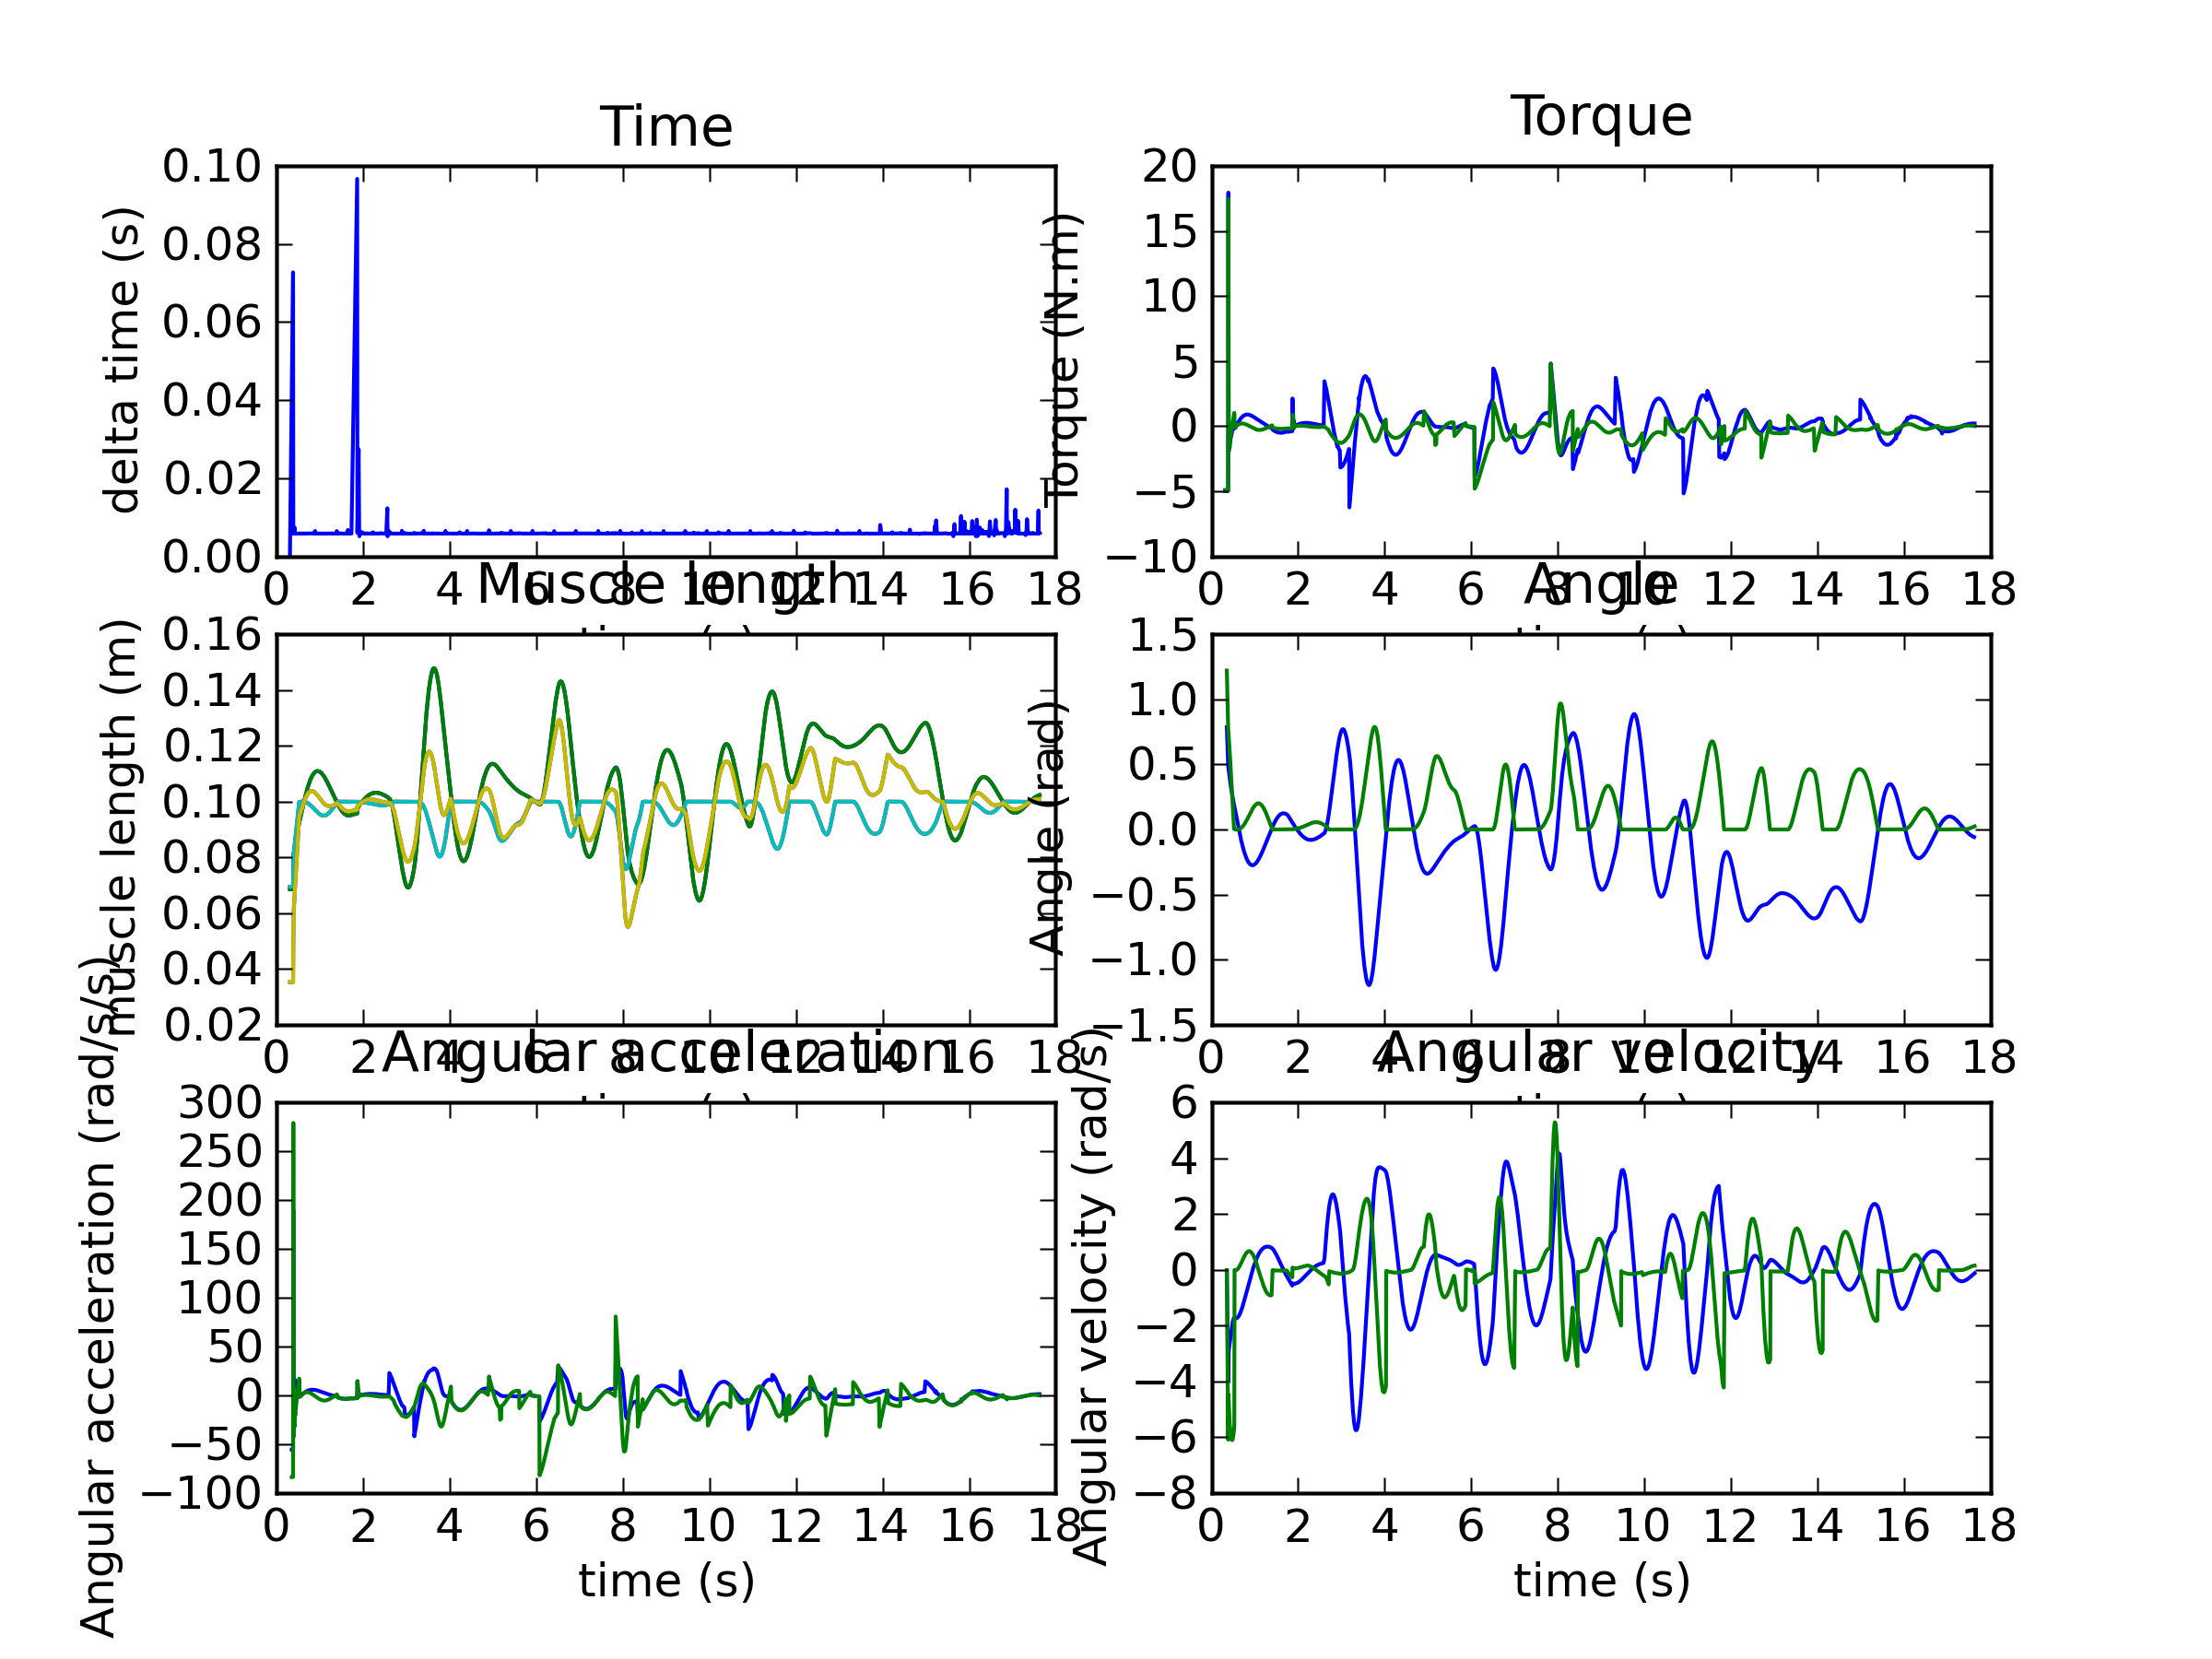
\includegraphics[width=.50\linewidth]{fig/pyarm2}}~~~
%    \subfigure{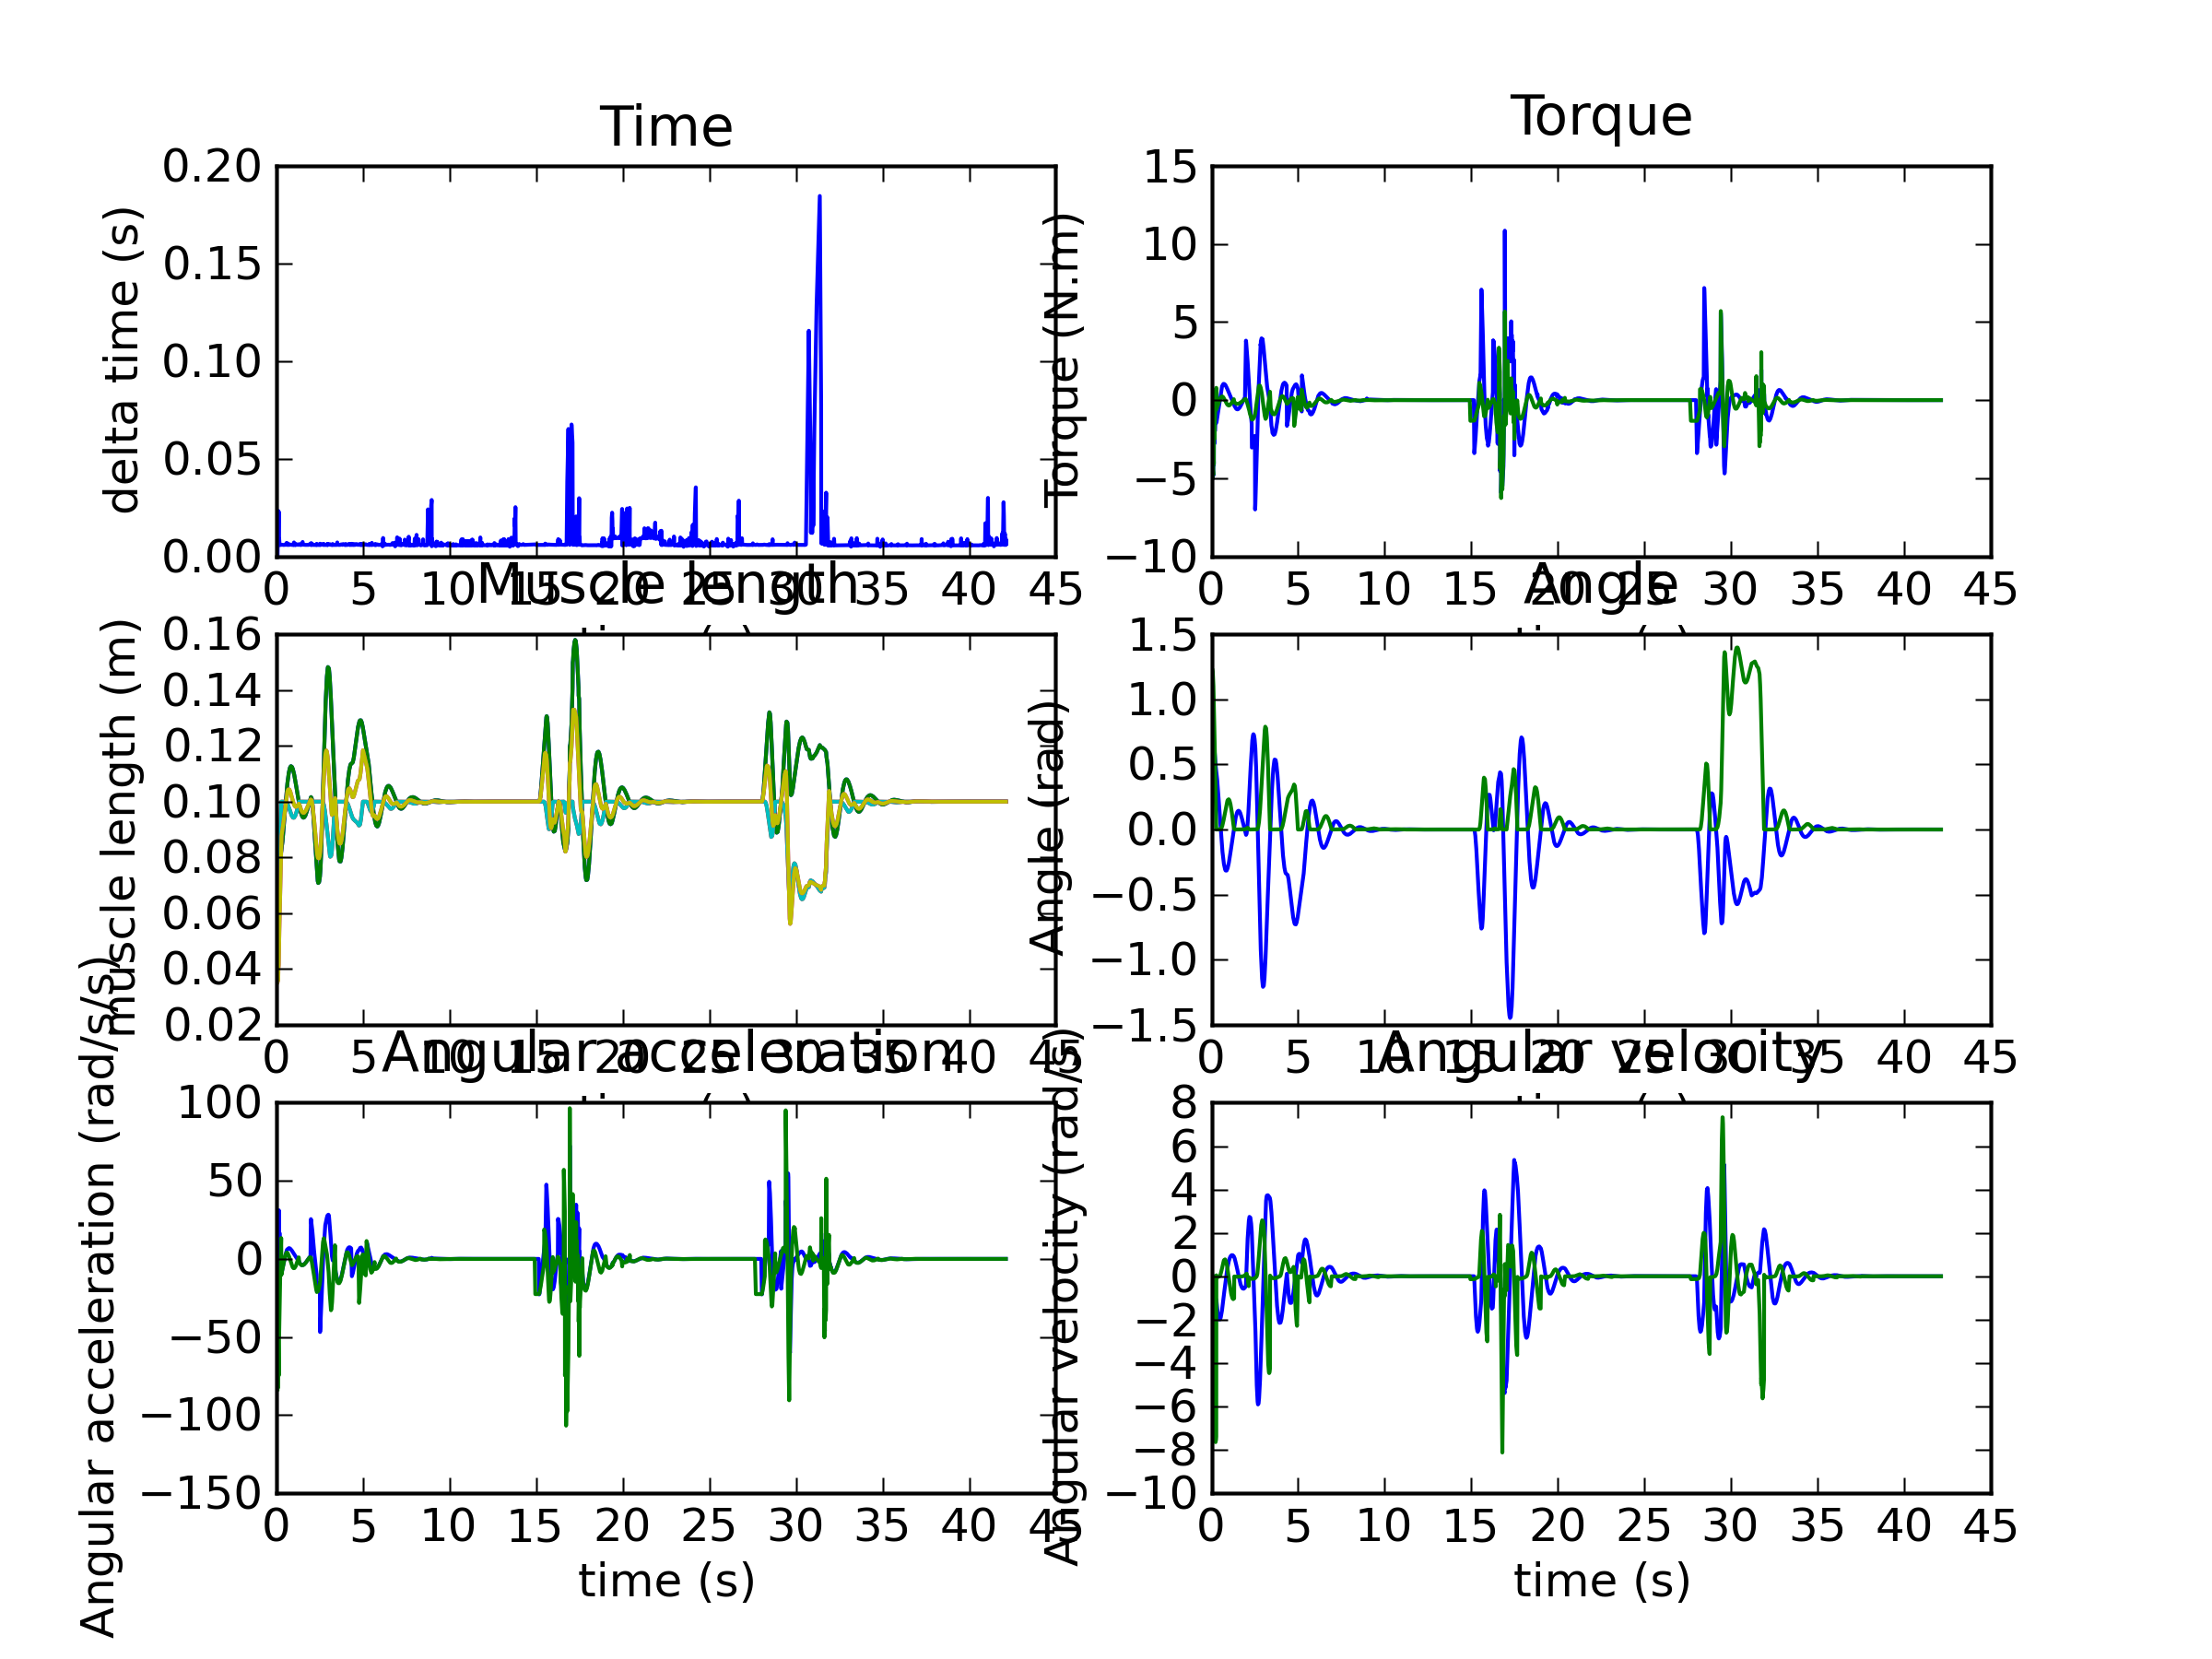
\includegraphics[width=.50\linewidth]{fig/pyarm3}}~~~
%\end{figure}

\paragraph{}
Le simulateur est composé de 5 modules :
\begin{itemize}
    \item Filtre sur signal d'entrée
    \item Modèle de bras
    \begin{itemize}
        \item Cinématique directe
        \item Dynamique directe
    \end{itemize}
    \item Modèle de muscle
    \begin{itemize}
        \item Cinématique inverse
        \item Dynamique directe
    \end{itemize}
\end{itemize}

\paragraph{}
\begin{center}
        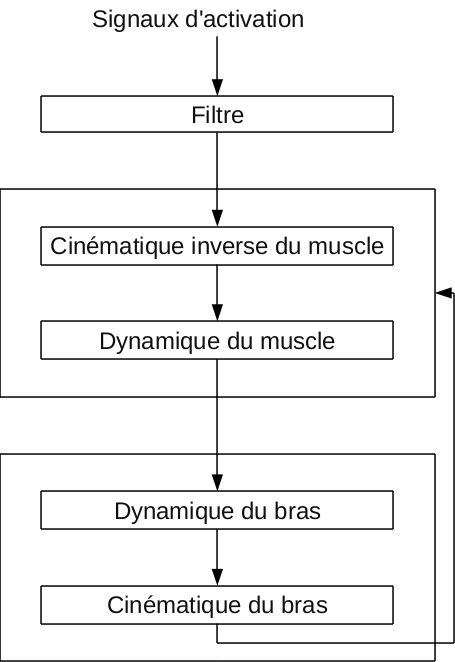
\includegraphics[width=.60\linewidth]{fig/modules}
\end{center}

%%%%%%%%%%%%%%%%%%%%%%%%%%%%%%%%%%%%%%%%%%%%%%%%%%%%%%%%%%%%%%%%%%%%%%%%%%%%%%%%

\section{Cinématique inverse du muscle}

\subsection{Résolution numérique par la méthode des différences finies du premier ordre}

Cette méthode de résolution numérique est la plus simple : elle se base sur la discrétisation de l'intervalle d'étude en un certain nombre de pas.

\paragraph{}
\begin{small}
\begin{tabular}{ll}
    $\vs{l_m}(\vs{q}) \in \mathbb{R}^6$                  & Longueur constatée des muscles $(m)$ \\
    $\vs{\dot{l_m}}(\vs{q}, \vs{\dot{q}}) \in \mathbb{R}^6$   & Vitesse de contraction des muscles $(m \cdot s^{-1})$ \\

    $\ms{A}(\vs{q}) \in \mathbb{R}^{6 \times 2}$   &  Matrice des bras de levier $(m)$\\
    $\vs{l_{m0}} \in \mathbb{R}^6$            &  Longueur des muscles quand les articulations sont d'angle nul $(m)$ \\
    $\vs{q} \in \mathbb{R}^2$                 &  Angle des articulations $(rad)$ \\
    $\vs{\dot{q}} \in \mathbb{R}^2$           &  Vitesse angulaire des articulations $(rad \cdot s^{-1})$ \\
\end{tabular}
\end{small}

\[\vs{l_m}(\vs{q}) = \vs{l_{m0}} - \ms{A}(\vs{q}) \vs{q}\]
\[\vs{\dot{l_m}}(\vs{q}, \vs{\dot{q}}) = \frac{\delta \vs{l_m}(\vs{q})}{\delta t}\]

\begin{center}
        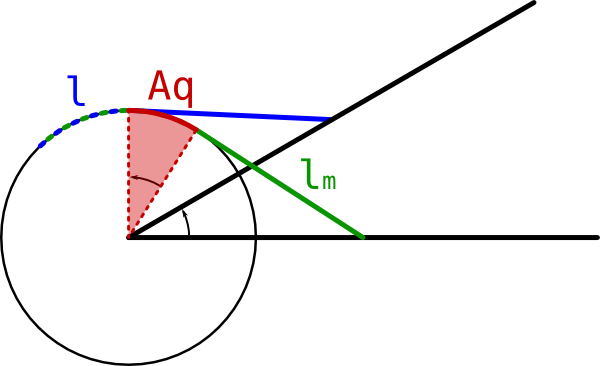
\includegraphics[width=.50\linewidth]{fig/muscle_length}
\end{center}

% TODO
Dans les modèles de Mitrovic et de Kambara, la longueur du bras de levier est constante.% Elle correspond au rayon ...
%Sous réserve que la longueur de l'arc soit toujours positive (...)
% TODO
    
\begin{figure}[h]
    \centering
    \subfigure{\includegraphics[width=.40\linewidth]{fig/moment_arm}}~~~
    \subfigure{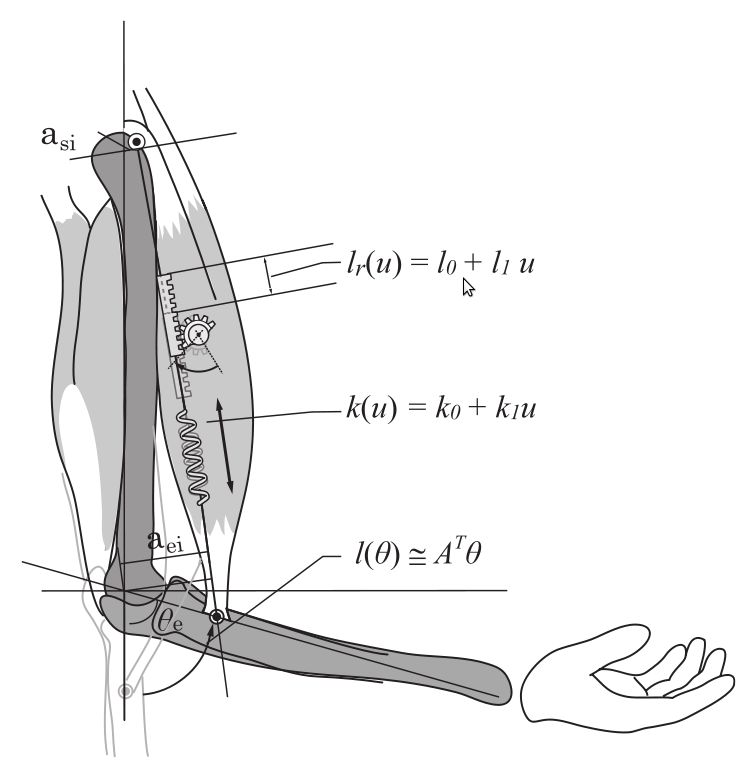
\includegraphics[width=.40\linewidth]{fig/arm_shin}}~~~
\end{figure}

\begin{footnotesize}
\begin{tabular*}{1.0\textwidth}{@{\extracolsep{\fill}}|l|r|r|r|r|r|r|}
    \hline
                            & Mitrovic &  &  & Kambara &  &  \\
    \hline
                            & $a_s$ & $a_e$ & $l_{m0}$ & $a_s$   &  $a_e$  & $l_{m0}$ \\
    \hline
    fléchisseur de l'épaule &  0.04 &     0 &    0.337 &    0.04 &      0  &  0.337 \\
    \hline
    extenseur de l'épaule   &  0.04 &     0 &    0.388 &   -0.04 &      0  &  0.388 \\
    \hline
    fléchisseur du coude    &     0 & 0.025 &    0.375 &       0 &  0.025  &  0.375 \\
    \hline
    extenseur du coude      &     0 & 0.025 &    0.315 &       0 & -0.025  &  0.315 \\
    \hline
    double fléchisseur      & 0.028 & 0.028 &    0.257 &   0.028 &  0.028  &  0.257 \\
    \hline
    double extenseur        & 0.035 & 0.035 &    0.256 &  -0.035 & -0.035  &  0.256 \\
    \hline
\end{tabular*}
\end{footnotesize}

\begin{figure}[h]
    \centering
    \subfigure{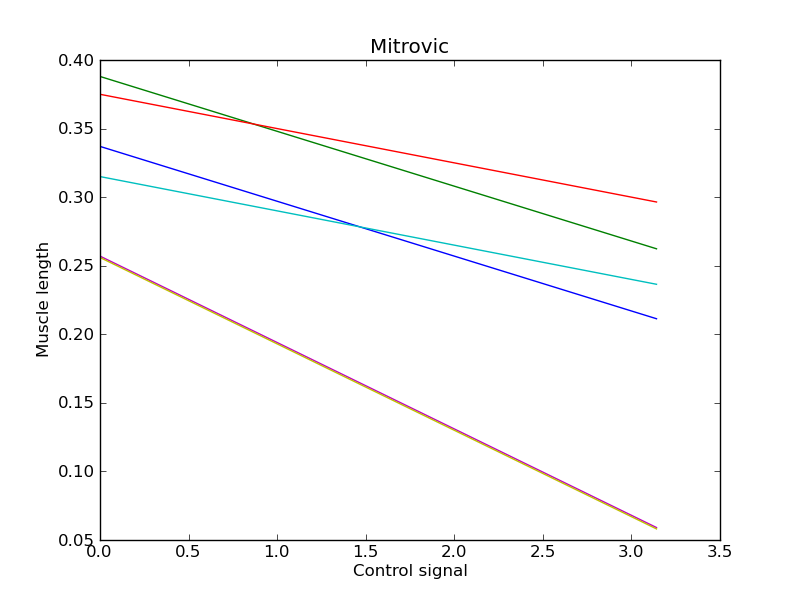
\includegraphics[width=.50\linewidth]{fig/muscle_Mitrovic_lm}}~~~
    \subfigure{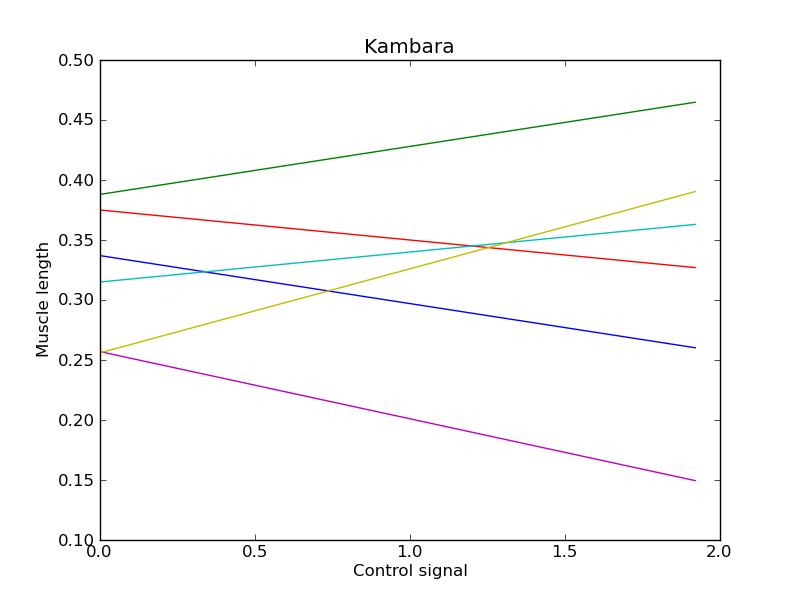
\includegraphics[width=.50\linewidth]{fig/muscle_Kambara_lm}}~~~
\end{figure}

%%%%%%%%%%%%%%%%%%%%%%%%%%%%%%%%%%%%%%%%%%%%%%%%%%%%%%%%%%%%%%%%%%%%%%%%%%%%%%%%

\section{Dynamique du muscle}

\subsection{Katayama (Mitrovic et Kambara)}

\paragraph{}
Mitrovic~:
\[ \vs{\tau} = -\ms{A}^T \vs{T}(\vs{l_m}, \vs{\dot{l_m}}, \vs{\tilde{u}}) \]
\[ \vs{T}(\vs{l_m}, \vs{\dot{l_m}}, \vs{\tilde{u}}) = \vs{k}(\vs{\tilde{u}})  \cdot (\vs{l_r}(\vs{\tilde{u}}) - \vs{l_m}) + \vs{\nu}(\vs{\tilde{u}}) \cdot \vs{\dot{l_m}} \]

\paragraph{}
Kambara~:
\[ \vs{\tau} = \ms{A}^T \vs{T}(\vs{l_m}, \vs{\dot{l_m}}, \vs{\tilde{u}}) \]
\[ \vs{T}(\vs{l_m}, \vs{\dot{l_m}}, \vs{\tilde{u}}) = -\vs{k}(\vs{\tilde{u}}) \cdot (\vs{l_r}(\vs{\tilde{u}}) - \vs{l_m}) + \vs{\nu}(\vs{\tilde{u}}) \cdot \vs{\dot{l_m}} \]

\paragraph{}
\begin{tabular}{lcl}
    $\vs{k}  (\vs{\tilde{u}})$  & = &  $\vs{k_0}    + \vs{k_1}    \cdot \vs{\tilde{u}}$ \\
    $\vs{\nu}(\vs{\tilde{u}})$  & = &  $\vs{\nu_0}  + \vs{\nu_1}  \cdot \vs{\tilde{u}}$ \\
    $\vs{l_r}(\vs{\tilde{u}})$  & = &  $\vs{l_{r0}} - \vs{l_{r1}} \cdot \vs{\tilde{u}}$ \\
\end{tabular}

\begin{figure}[h]
    \centering
    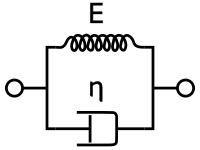
\includegraphics[width=.20\linewidth]{fig/Kelvin_Voigt_diagram}
    \caption{Kelvin-Voigt model}
\end{figure}

\paragraph{}
\begin{small}
\begin{tabular}{lcl}
    $\vs{\tau} \in \mathbb{R}^2$              & = & Couple total exercé sur les articulations $(N \cdot m)$ \\
    $\ms{A} \in \mathbb{R}^{6 \times 2}$      & = & Matrice des bras de levier $(m)$ \\
    $\vs{T}(\vs{l_m}, \vs{\dot{l_m}}, \vs{\tilde{u}}) \in \mathbb{R}^6$  & = & Tension exercée par les muscles $(N)$ \\
    \\
    $\vs{k}(\vs{\tilde{u}}) \cdot (\vs{l_r}(\vs{\tilde{u}}) - \vs{l_m})$ & = & Force élastique des muscles (raideur $\cdot$ étirement) \\
    \\

    $\vs{k}(\vs{\tilde{u}}) \in \mathbb{R}^6$      & = & Raideur des muscles \\
    $\vs{k_0} \in \mathbb{R}^6$               & = & Raideur intrinsèque des muscles $(N/m)$ \\
    $\vs{k_1} \in \mathbb{R}^6$               & = & Coefficient de variation de l'élasticité des muscles $(N/m)$ \\
    \\

    $\vs{\nu}(\vs{\tilde{u}}) \in \mathbb{R}^6$    & = & Viscosité des muscles \\
    $\vs{\nu_0} \in \mathbb{R}^6$             & = & Viscosité intrinsèque des muscles $(N \cdot s/m)$ \\
    $\vs{\nu_1} \in \mathbb{R}^6$             & = & Coefficient de variation de la viscosité des muscles $(N \cdot s/m)$ \\
    \\

    $\vs{l_r}(\vs{\tilde{u}}) \in \mathbb{R}^6$    & = & Longueur des muscles au repos pour un taux d'activation donné $(m)$ \\
    $\vs{l_{r0}} \in \mathbb{R}^6$            & = & Longueur intrinsèque des muscles au repos $(m)$ \\
    $\vs{l_{r1}} \in \mathbb{R}^6$            & = & Coefficient de variation de la longueur des muscles au repos $(m)$ \\
    \\

    $\vs{l_m} \in \mathbb{R}^6$               & = & Longueur constatée des muscles $(m)$ \\
    $\vs{l_{m0}} \in \mathbb{R}^6$            & = & Longueur des muscles quand les articulations sont d'angle nul $(m)$ \\
    \\

    $\vs{u} \in \mathbb{R}^6$                 & = & Signaux d'activation des muscles $(u_i \in [0;1])$ \\
    $\vs{\tilde{u}} \in \mathbb{R}^6$         & = & Signaux d'activation filtrés $(\tilde{u_i} \in [0;1])$ \\
\end{tabular}
\end{small}

\paragraph{}
Mitrovic \cite{katayama1993} (p.356-357)~: 
\[
\ms{A} =
\begin{pmatrix}
    0.04 & 0.04 & 0     & 0     & 0.028 & 0.035 \\
    0    & 0    & 0.025 & 0.025 & 0.028 & 0.035 \\
\end{pmatrix}^T
\]

\begin{footnotesize}
\begin{tabular*}{1.0\textwidth}{@{\extracolsep{\fill}}|l|r|r|r|r|r|r|}
    \hline
                            & $k_0$ & $k_1$  & $\nu_0$ & $\nu_1$ & $l_{r1}$               & $l_{m0} - l_{r0}$ \\
    \hline                                            
    fléchisseur de l'épaule & 810.8 & 1621.6 & 54.1    & 108.1   & $-3.49 \cdot 10^{-2}$  & $  9.08 \cdot 10^{-2}$ \\
    \hline
    extenseur de l'épaule   & 810.8 & 1621.6 & 54.1    & 108.1   & $ 3.49 \cdot 10^{-2}$  & $ -2.79 \cdot 10^{-2}$ \\
    \hline
    fléchisseur du coude    & 810.8 & 1621.6 & 54.1    & 108.1   & $-2.18 \cdot 10^{-2}$  & $  5.67 \cdot 10^{-2}$ \\
    \hline
    extenseur du coude      & 810.8 & 1621.6 & 54.1    & 108.1   & $ 2.18 \cdot 10^{-2}$  & $  0.44 \cdot 10^{-2}$ \\
    \hline
    double fléchisseur      & 810.8 & 1621.6 & 54.1    & 108.1   & $-5.50 \cdot 10^{-2}$  & $ 14.29 \cdot 10^{-2}$ \\
    \hline
    double extenseur        & 810.8 & 1621.6 & 54.1    & 108.1   & $ 5.50 \cdot 10^{-2}$  & $ -1.34 \cdot 10^{-2}$ \\
    \hline
\end{tabular*}
\end{footnotesize}

\paragraph{}
Kambara  \cite{kambara2009} (p.359-360)~:
\[
\ms{A} =
\begin{pmatrix}
    0.04 & -0.04 & 0     & 0      & 0.028 & -0.035 \\
    0    & 0     & 0.025 & -0.025 & 0.028 & -0.035 \\
\end{pmatrix}^T
\]

\begin{small}
\begin{tabular*}{1.0\textwidth}{@{\extracolsep{\fill}}|l|r|r|r|r|r|r|}
    \hline
                            & $k_0$  & $k_1$  & $\nu_0$ & $\nu_1$ & $l_{r1}$ & $l_{m0} - l_{r0}$ \\
    \hline
    fléchisseur de l'épaule & 1000   & 3000   & 50      & 100     & 0.15     & 0.077 \\
    \hline
    extenseur de l'épaule   & 1000   & 2000   & 50      & 100     & 0.15     & 0.128 \\
    \hline
    fléchisseur du coude    & 600    & 1400   & 50      & 100     & 0.15     & 0.100 \\
    \hline
    extenseur du coude      & 600    & 1200   & 50      & 100     & 0.15     & 0.040 \\
    \hline
    double fléchisseur      & 300    & 600    & 50      & 100     & 0.15     & 0.020 \\
    \hline
    double extenseur        & 300    & 600    & 50      & 100     & 0.15     & 0.019 \\
    \hline
\end{tabular*}
\end{small}

\begin{figure}[h!]
    \centering
    \subfigure{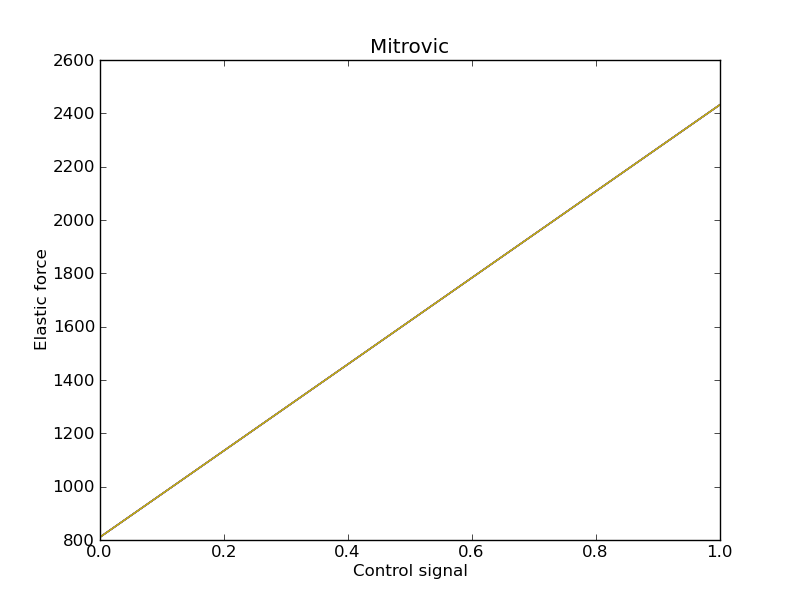
\includegraphics[width=.50\linewidth]{fig/muscle_Mitrovic_k}}~~~
    \subfigure{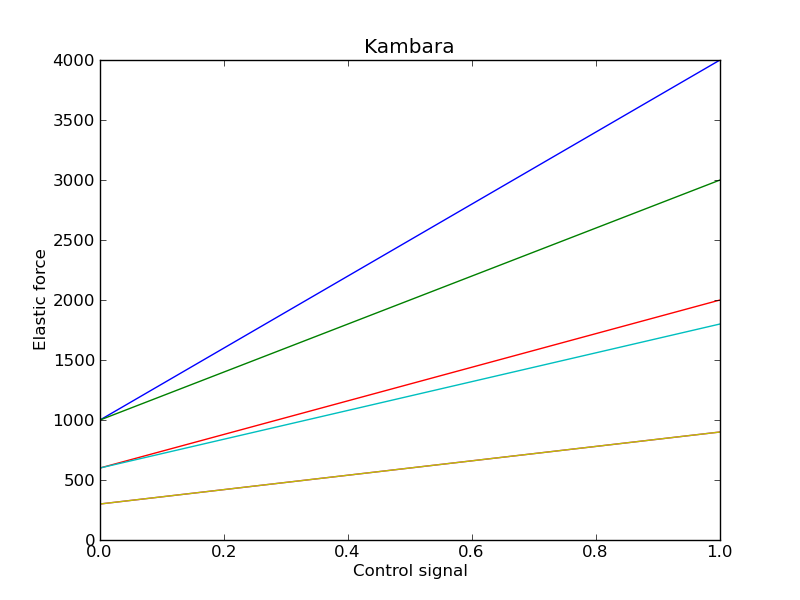
\includegraphics[width=.50\linewidth]{fig/muscle_Kambara_k}}~~~
\end{figure}

\begin{figure}[h!]
    \centering
    \subfigure{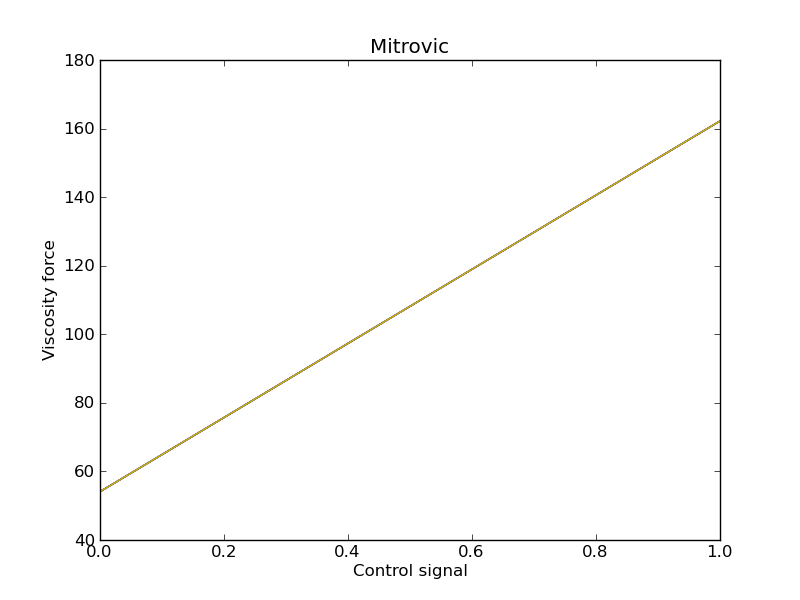
\includegraphics[width=.50\linewidth]{fig/muscle_Mitrovic_v}}~~~
    \subfigure{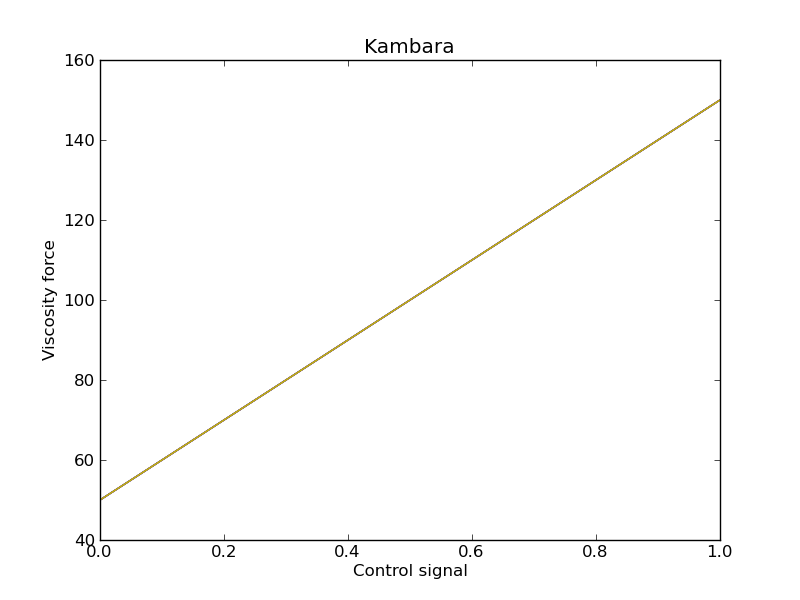
\includegraphics[width=.50\linewidth]{fig/muscle_Kambara_v}}~~~
\end{figure}

\begin{figure}[h!]
    \centering
    \subfigure{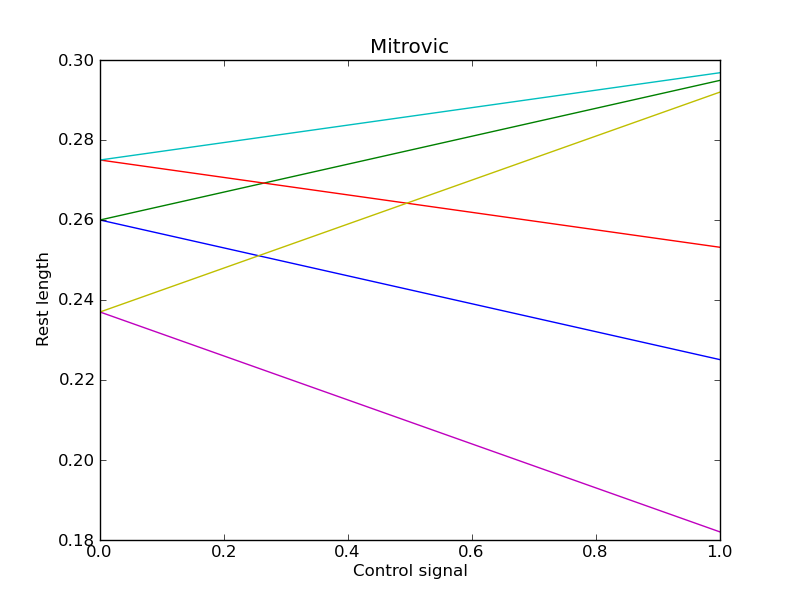
\includegraphics[width=.50\linewidth]{fig/muscle_Mitrovic_lr}}~~~
    \subfigure{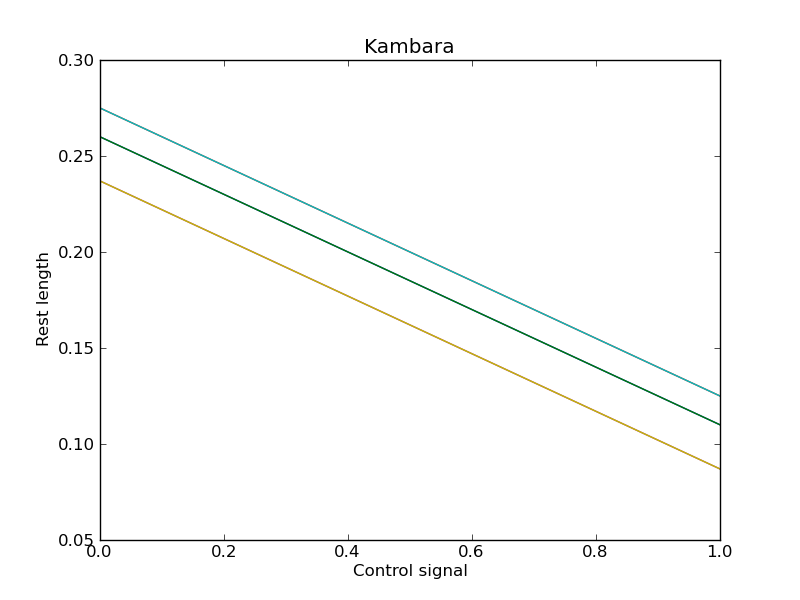
\includegraphics[width=.50\linewidth]{fig/muscle_Kambara_lr}}~~~
\end{figure}

%%%%%%%%

\subsection{Brown (Weiwei)}

\begin{figure}[h]
    \centering
    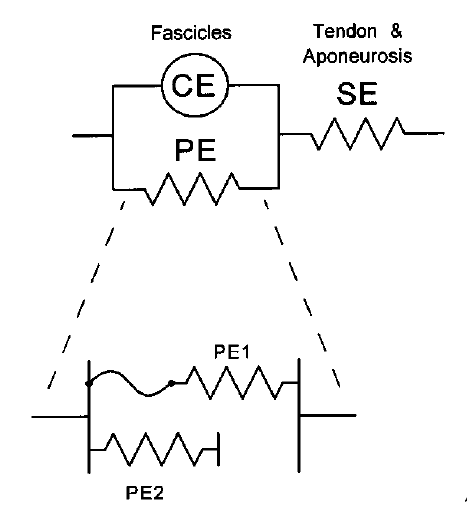
\includegraphics[width=.30\linewidth]{fig/brown}
\end{figure}

\begin{tabular}{ll}
    $CE$  & Éléments contractiles \\
    $SE$  & Élasticité des tendons (ignorée) \\
    $PE$  & Élasticité du muscle \\
    $PE1$ & Résistance à l'étirement du muscle passif \\
    $PE2$ & Résistance à la compression du muscle actif \\
    \\

    $\vs{\tau_i} \in \mathbb{R}^2$                   & Couple total exercé sur les articulations par le muscle $i$ $(N \cdot m)$ \\
    $\vs{a_i}(\vs{q}) \in \mathbb{R}^2$              & Bras de levier du muscle $i$ sur les deux articulations $(c_1 + c_2 \cos (c_3 \vs{q}))$ $(m)$ \\
    $T_i(l_m, \dot{l_m}, \tilde{u}) \in \mathbb{R}$  & Tension exercée par le muscle $i$ $(N)$ \\
    \\

    $f_a(\tilde{u}, l_m) \in \mathbb{R}$   & Relation activation-fréquence \\
    $f_l(l_m) \in \mathbb{R}$              & Relation force-longueur \\
    $f_v(l_m, \dot{l_m}) \in \mathbb{R}$   & Relation force-vitesse \\
    $f_e(l_m) \in \mathbb{R}$              & Force élastique du muscle \\ % TODO ???
    \\

    $l_m \in \mathbb{R}$                   & Longueur constatée du muscle $i$ $(m)$ \\
    $\dot{l_m} \in \mathbb{R}$             & Vitesse de contraction du muscle $i$ $(m \cdot s^{-1})$ \\
    \\

    $u \in \mathbb{R}$                     & Signaux d'activation du muscle $i$ $(u_i \in [0;1])$ \\
    $\tilde{u} \in \mathbb{R}$             & Signaux d'activation filtrés $(\tilde{u_i} \in [0;1])$ \\
\end{tabular}

\[
\left\{
\begin{tabular}{lcl}
    $\vs{\tau_{total}}$ & = & $\sum_{i = 0}^{6} \vs{\tau_i}$ \\
    $\vs{\tau_i}$ & = & $\vs{a_i}(\vs{q}) T_i(l_m, \dot{l_m}, \tilde{u})$ \\
    \\
    $T_i(l_m, \dot{l_m}, \tilde{u})$ & = & $f_a(l_m, \tilde{u})(f_e(l_m) + f_l(l_m) f_v(l_m, \dot{l_m}))$ \\
    $f_a(l_m, \tilde{u})$          & = & $1 - \exp \left(- \left(\frac{\tilde{u}}{0.56 n_f(l_m)}\right)^{n_f(l_m)}\right)$ \\
    $n_f(l_m)$                     & = & $2.11 + 4.16 \left(\frac{1}{l_m} - 1\right)$ \\
    $f_l(l_m)$                     & = & $\exp \left(-\left|\frac{l_m^{1.93} - 1}{1.03}\right|^{1.87}\right)$ \\
    $f_v(l_m, \dot{l_m})$          & = & 
        $\left\{ 
        \begin{array}{l}
            \frac{-5.72 - \dot{l_m}}{-5.72 + (1.38 + 2.09 l_m) \dot{l_m}}, \dot{l_m} \leq 0 \\
            \frac{0.62 - \left(-3.12 + 4.21 l_m - 2.67 l_m^2\right) \dot{l_m}}{0.62 + \dot{l_m}}, \dot{l_m} > 0 \\
        \end{array}
        \right.$ \\
    $f_e(l_m)$                     & = & $-0.02 \exp(13.8 - 18.7 l_m)$ \\
\end{tabular}
\right.
\]

\begin{figure}[h]
    \centering
    \subfigure[$f_a$ : activation-fréquence]{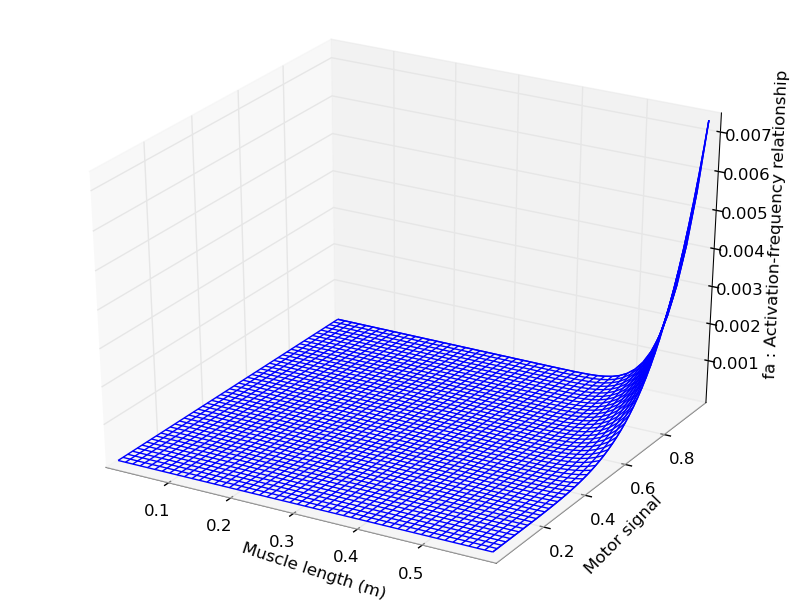
\includegraphics[width=.40\linewidth]{fig/muscle_Weiwei_fa}}~~~
    \subfigure[$n_f$]{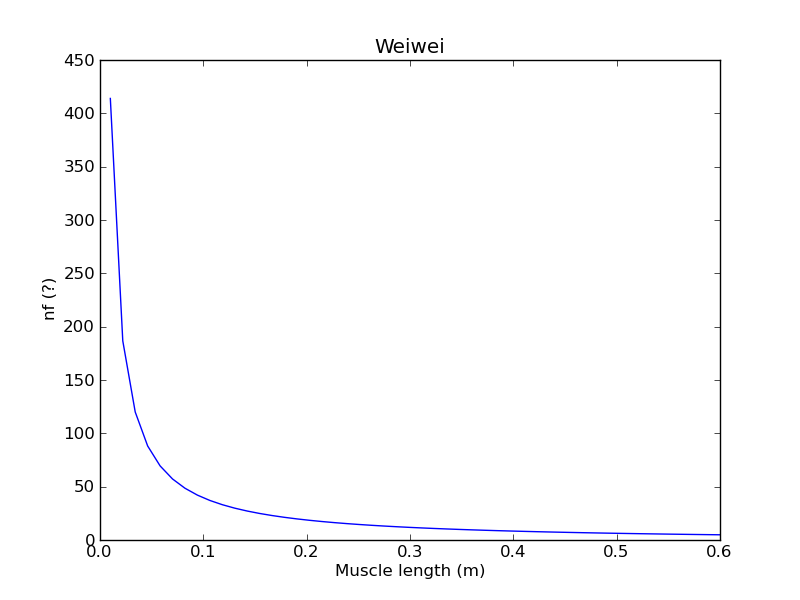
\includegraphics[width=.40\linewidth]{fig/muscle_Weiwei_nf}}~~~
\end{figure}

\begin{figure}[h]
    \centering
    \subfigure[$f_l$ : force-longueur]{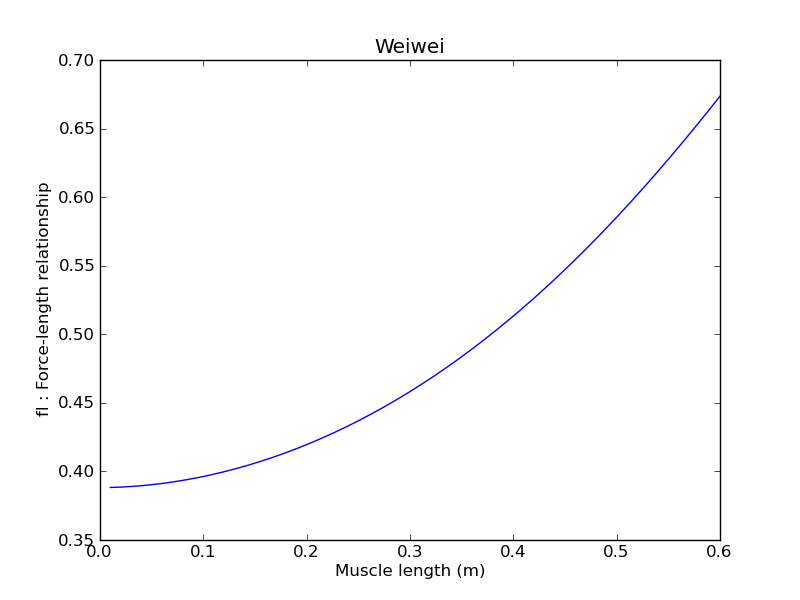
\includegraphics[width=.40\linewidth]{fig/muscle_Weiwei_fl}}~~~
    \subfigure[$f_v$ : force-vitesse]{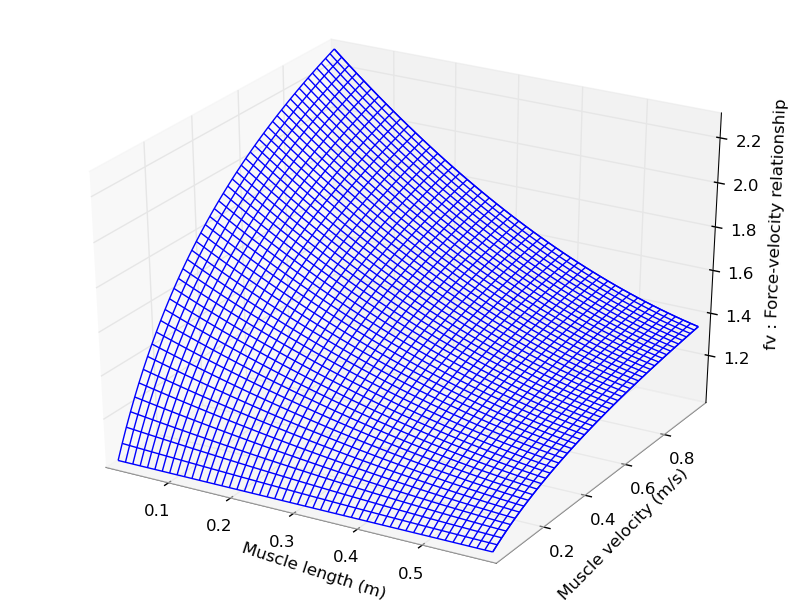
\includegraphics[width=.40\linewidth]{fig/muscle_Weiwei_fv}}~~~
\end{figure}

\begin{figure}[h]
    \centering
    \subfigure[$f_l$ : force élastique]{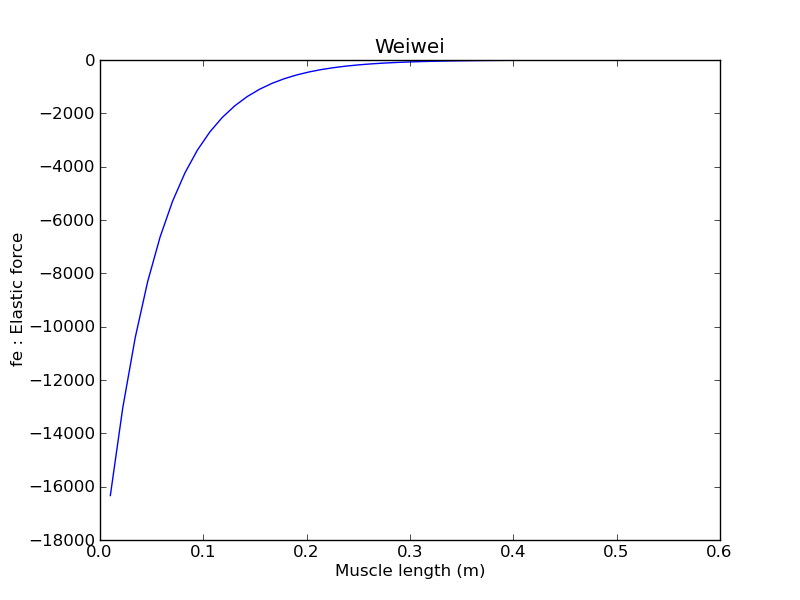
\includegraphics[width=.40\linewidth]{fig/muscle_Weiwei_fe}}
\end{figure}

%%%%%%%%%%%%%%%%%%%%%%%%%%%%%%%%%%%%%%%%%%%%%%%%%%%%%%%%%%%%%%%%%%%%%%%%%%%%%%%%

\section{Dynamique du bras}

%%%%%%%%

\subsection{Cas général}

\begin{tabular}{ll}
    $\ms{M}(\vs{q}) \in \mathbb{R}^{2 \times 2}$  & Matrice des moments d'inertie \\ % TODO
    $\vs{C}(\vs{q}, \vs{\dot{q}}) \in \mathbb{R}^{2}$  & Force de Coriolis et force centripète \\
    $\vs{B}(\vs{\dot{q}}) \in \mathbb{R}^{2}$     & Force de viscosité et de friction \\ % TODO
    $\vs{G}(\vs{q}) \in \mathbb{R}^{2}$           & Force de gravité \\
    $\vs{\tau} \in \mathbb{R}^{2}$           & Couple total exercé sur les articulations ($N \cdot m$) \\
    $\vs{\ddot{q}} \in \mathbb{R}^{2}$       & Accélération angulaire des articulations ($rd \cdot s^{-2}$) \\
    $\vs{\dot{q}} \in \mathbb{R}^{2}$        & Vitesse angulaire des articulations ($rd \cdot s^{-1}$)\\
    $\vs{q} \in \mathbb{R}^{2}$              & Angle des articulations ($rd$)\\
\end{tabular}

\paragraph{}
Dynamique inverse~:
\[\vs{\tau} = \ms{M}(\vs{q})\vs{\ddot{q}} + \vs{C}(\vs{q}, \vs{\dot{q}}) + \vs{B}(\vs{\dot{q}}) + \vs{G}(\vs{q})\]

\paragraph{}
Dynamique directe~:
\[\Leftrightarrow \vs{\ddot{q}} = \ms{M}(\vs{q})^{-1} (\vs{\tau} - \vs{C}(\vs{q}, \vs{\dot{q}}) - \vs{B}(\vs{\dot{q}}) - \vs{G}(\vs{q}))\]

%%%%%%%%

\subsection{Modèles étudiés}

\paragraph{}
\begin{tabular}{|c|l|l|}
    \hline
    Mitrovic & $\vs{\tau} = \ms{M}(\vs{q})\vs{\ddot{q}} + \vs{C}(\vs{q}, \vs{\dot{q}})$
             & $\vs{\ddot{q}} = \ms{M}(\vs{q})^{-1} (\vs{\tau} - \vs{C}(\vs{q}, \vs{\dot{q}}))$ \\
    \hline
    Kambara  & $\vs{\tau} = \ms{M}(\vs{q})\vs{\ddot{q}} + \vs{C}(\vs{q}, \vs{\dot{q}}) + \vs{G}(\vs{q})$
             & $\vs{\ddot{q}} = \ms{M}(\vs{q})^{-1} (\vs{\tau} - \vs{C}(\vs{q}, \vs{\dot{q}}) - \vs{G}(\vs{q}))$ \\
    \hline
    Weiwei   & $\vs{\tau} = \ms{M}(\vs{q})\vs{\ddot{q}} + \vs{C}(\vs{q}, \vs{\dot{q}}) + \vs{B}(\vs{\dot{q}})$
             & $\vs{\ddot{q}} = \ms{M}(\vs{q})^{-1} (\vs{\tau} - \vs{C}(\vs{q}, \vs{\dot{q}}) - \vs{B}(\vs{\dot{q}}))$ \\
    \hline
\end{tabular}

\begin{center}
        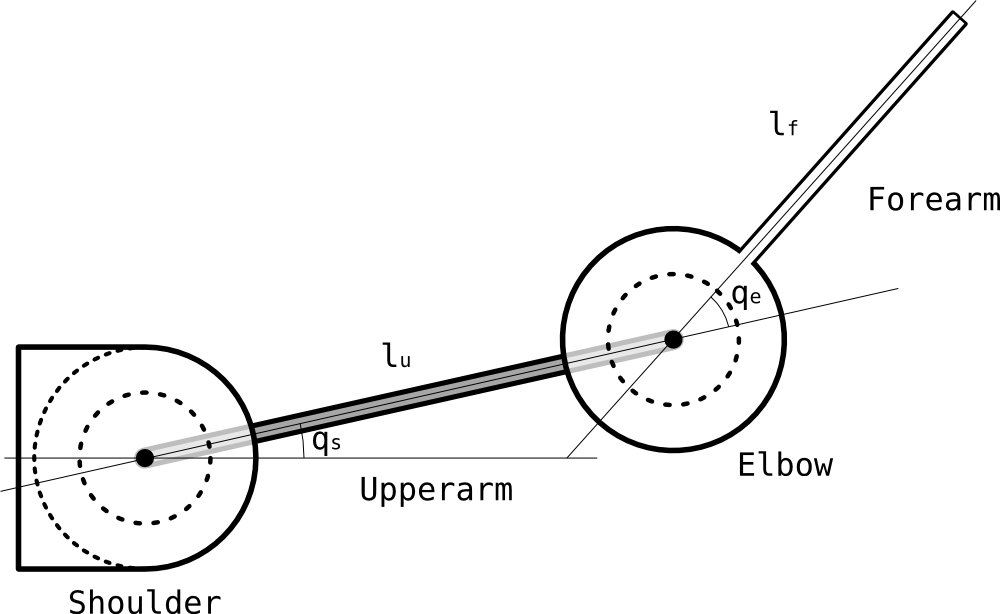
\includegraphics[width=.80\linewidth]{fig/arm}
\end{center}

\paragraph{}
\begin{tabular}{ll}
    $m_i$      & Masse du membre $i$ ($kg$) \\
    $l_i$      & Longueur du membre $i$ ($m$) \\
    $\gamma_i$ & Distance séparant le centre de l'articulation au centre de masse du membre $i$ ($m$) \\
    $\iota_j$  & Moment d'inertie de l'articulation $j$ ($kg \cdot m^2$) \\
    $g$        & Champ de pesanteur ($m \cdot s^{-2}$) \\
\end{tabular}

\paragraph{}
\begin{tabular}{ll}
    Indices & \\
    $u$ & Bras (supérieur)\\
    $f$ & Avant-bras\\
    $s$ & Épaule\\
    $e$ & Coude\\
\end{tabular}

\paragraph{}
\begin{tabular}{lcl}
    $\ms{M}(\vs{q})$ & = &
    $
    \begin{pmatrix}
        f_1 + 2 f_2 \cos(q_e)  & f_3 + f_2 \cos(q_e) \\
        f_3 + f_2 \cos(q_e) & f_3 \\
    \end{pmatrix}
    $ \\

    $\vs{C}(\vs{q}, \vs{\dot{q}})$ & = &
    $
    \begin{pmatrix}
        -\dot{q}_e (2 \dot{q}_s + \dot{q}_e) \\
        \dot{q}_s^2 \\
    \end{pmatrix}
    f_2 \sin(q_e)
    $\\

    $\vs{B}(\vs{\dot{q}})$ & = &
    $
    \begin{pmatrix}
        0.05  & 0.025 \\
        0.025 & 0.05 \\
    \end{pmatrix}
    \vs{\dot{q}}
    $\\

    $\vs{G}(\vs{q})$ & = &
    $
    \begin{pmatrix}
        m_u g  \gamma_u \cos(q_s) + m_f g (l_u \cos(q_s) + \gamma_f \cos(q_s + q_e)) \\
        m_f g  \gamma_f \cos(q_s + q_e) \\
    \end{pmatrix}
    $ \\

    \\
    $f_1$ & = & $\iota_s + \iota_e + m_f l_u^2$ \\
    $f_2$ & = & $m_f l_u \gamma_f$ \\
    $f_3$ & = & $\iota_e$ \\
\end{tabular}

\paragraph{}
\begin{small}
\begin{tabular}{|c|c|c|c|c|c|c|c|c|c|}
    \hline
             & $m_u$  & $m_f$  & $l_u$ & $l_f$  & $\gamma_u$ & $\gamma_f$ & $\iota_s$            & $\iota_e$            & $g$ \\
    \hline
    Mitrovic \cite{katayama1993} (p.356) 
             & $1.59$ & $1.44$ & $0.3$ & $0.35$ & $0.18$     & $0.21$     & $4.77 \cdot 10^{-2}$ & $5.88 \cdot 10^{-2}$ & - \\
    \hline
    Kambara  \cite{kambara2009} (p.359)
             & $1.59$ & $1.44$ & $0.3$ & $0.35$ & $0.18$     & $0.21$     & $6.78 \cdot 10^{-2}$ & $7.99 \cdot 10^{-2}$ & N/C \\
    \hline
    Weiwei   \cite{li2006} (p.23)
             & $1.4$  & $1.1$  & $0.3$ & $0.33$ & $0.11$     & $0.16$     & $2.5 \cdot 10^{-2}$  & $4.5 \cdot 10^{-2}$  & - \\
    \hline
\end{tabular}
\end{small}

\begin{figure}[h]
    \centering
    \subfigure{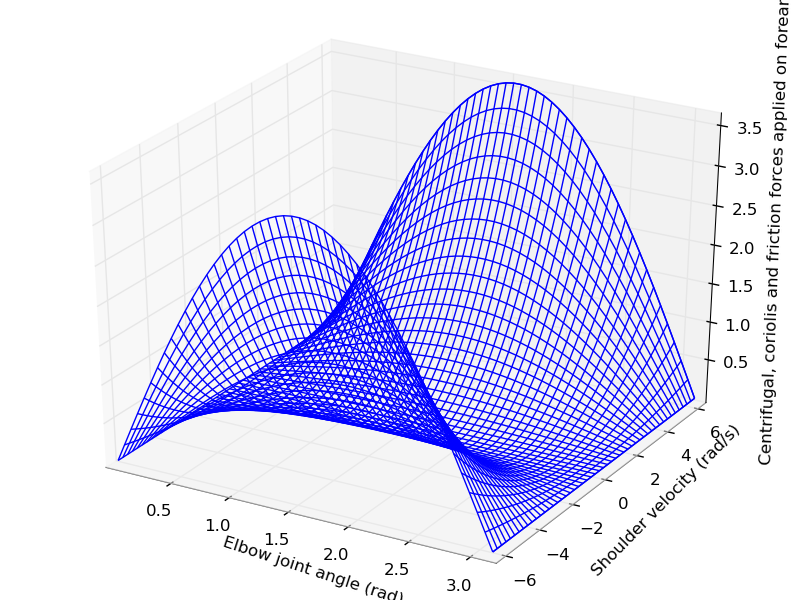
\includegraphics[width=.50\linewidth]{fig/arm_Mitrovic_c_forearm}}~~~
    \subfigure{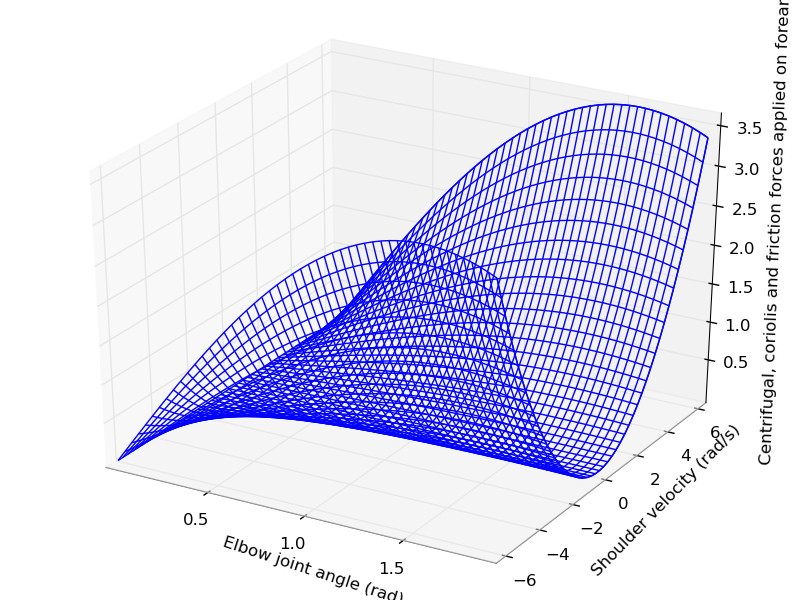
\includegraphics[width=.50\linewidth]{fig/arm_Kambara_c_forearm}}~~~
\end{figure}

%%%%%%%%%%%%%%%%%%%%%%%%%%%%%%%%%%%%%%%%%%%%%%%%%%%%%%%%%%%%%%%%%%%%%%%%%%%%%%%%

\section{Cinématique du bras}

\subsection{Résolution numérique par la méthode des différences finies du premier ordre}

Cette méthode de résolution numérique est la plus simple : elle se base sur la discrétisation de l'intervalle d'étude en un certain nombre de pas.

\[\dot{q} = \delta \ddot{q} \cdot \delta t\]
\[q = \delta \dot{q} \cdot \delta t\]

%%%%%%%%%%%%%%%%%%%%%%%%%%%%%%%%%%%%%%%%%%%%%%%%%%%%%%%%%%%%%%%%%%%%%%%%%%%%%%%%

\chapter{Apprentissage du contrôle moteur}

%%%%%%%%%%%%%%%%%%%%%%%%%%%%%%%%%%%%%%%%%%%%%%%%%%%%%%%%%%%%%%%%%%%%%%%%%%%%%%%%

\chapter{Annexe}

\section{Modèle du bras}

%%%%%%%%

\subsection{Mitrovic}
Écriture originale \cite{katayama1993} (p.355).

\begin{align*}
    \begin{pmatrix}
        \tau_s \\
        \tau_e \\
    \end{pmatrix} =
    & \begin{pmatrix}
        \iota_s + \iota_e + m_f l_u^2 + 2 m_f l_u \gamma_f \cos(q_e)  &  \iota_e + m_f l_u \gamma_f \cos(q_e) \\
        \iota_e + m_f l_u \gamma_f \cos(q_e)  &  \iota_e\\
    \end{pmatrix}
    \begin{pmatrix}
        \ddot{q}_s \\
        \ddot{q}_e \\
    \end{pmatrix}\\
    & + m_f l_u \gamma_f \sin(q_e)
    \begin{pmatrix}
        -2 \dot{q}_e  &  -\dot{q}_e \\
        \dot{q}_s     &  0\\
    \end{pmatrix}
    \begin{pmatrix}
        \dot{q}_s \\
        \dot{q}_e \\
    \end{pmatrix}
\end{align*}

$
\Leftrightarrow 
\left \{
    \begin{tabular}{rcl}
        $\vs{\tau}$ & = &
        $\ms{M}(\vs{q})\vs{\ddot{q}} + \vs{C}(\vs{q}, \vs{\dot{q}})$ \\

        $\ms{M}(\vs{q})$
        & = &
        $
        \begin{pmatrix}
            \iota_s + \iota_e + m_f l_u^2 + 2 m_f l_u \gamma_f \cos(q_e)  &  \iota_e + m_f l_u \gamma_f \cos(q_e) \\
            \iota_e + m_f l_u \gamma_f \cos(q_e)  &  \iota_e\\
        \end{pmatrix}
        $
        \\

        $\vs{C}(\vs{q}, \vs{\dot{q}})$
        & = &
        $
        m_f l_u \gamma_f \sin(q_e)
        \begin{pmatrix}
            -2 \dot{q}_e  &  -\dot{q}_e \\
            \dot{q}_s     &  0\\
        \end{pmatrix}
        \begin{pmatrix}
            \dot{q}_s \\
            \dot{q}_e \\
        \end{pmatrix}
        $
        \\
    \end{tabular}
\right .
$

$
\Leftrightarrow 
\left \{
    \begin{tabular}{rcl}
        $\vs{\tau}$ & = &
        $\ms{M}(\vs{q})\vs{\ddot{q}} + \vs{C}(\vs{q}, \vs{\dot{q}})$ \\

        $\ms{M}(\vs{q})$ & = &
        $
        \begin{pmatrix}
            f_1 + 2 f_2 \cos(q_e)  & f_3 + f_2 \cos(q_e) \\
            f_3 + f_2 \cos(q_e) & f_3 \\
        \end{pmatrix}
        $ \\

        $\vs{C}(\vs{q}, \vs{\dot{q}})$ & = &
        $
        \begin{pmatrix}
            -\dot{q}_e (2 \dot{q}_s + \dot{q}_e) \\
            \dot{q}_s^2 \\
        \end{pmatrix}
        f_2 \sin(q_e)
        $\\

        $f_1$ & = & $\iota_s + \iota_e + m_f l_u^2$ \\
        $f_2$ & = & $m_f l_u \gamma_f$ \\
        $f_3$ & = & $\iota_e$ \\
    \end{tabular}
\right .
$

%%%%%%%%

\subsection{Kambara}
Écriture originale \cite{kambara2009} (p.360).

\begin{align*}
    \begin{pmatrix}
        \tau_s \\
        \tau_e \\
    \end{pmatrix}
    & = \begin{pmatrix}
        M_{11}\ddot{q}_s + M_{12}\ddot{q}_e + h_{122}\dot{q}_e^2 + 2h_{112}\dot{q}_s\dot{q}_e + g_1 \\
        M_{21}\ddot{q}_s + M_{22}\ddot{q}_e + h_{211}\dot{q}_s^2 + g_2 \\
    \end{pmatrix}\\
    & = \begin{pmatrix}
        M_{11}\ddot{q}_s + M_{12}\ddot{q}_e \\
        M_{21}\ddot{q}_s + M_{22}\ddot{q}_e \\
    \end{pmatrix} +
    \begin{pmatrix}
        h_{122}\dot{q}_e^2 + 2h_{112}\dot{q}_s\dot{q}_e \\
        h_{211}\dot{q}_s^2 \\
    \end{pmatrix} +
    \begin{pmatrix}
        g_1 \\
        g_2 \\
    \end{pmatrix}\\
    & = \ms{M}(\vs{q}) \vs{\ddot{q}} + \vs{C}(\vs{q}, \vs{\dot{q}}) + \vs{G}(\vs{q})
\end{align*}

\paragraph{}
\begin{tabular}{lcl}
    $\ms{M}(\vs{q})$ & = &
    $
    \begin{pmatrix}
        M_{11} & M_{12} \\
        M_{21} & M_{22} \\
    \end{pmatrix}
    $ \\

    $\vs{C}(\vs{q}, \vs{\dot{q}})$ & = &
    $
    \begin{pmatrix}
        -f_2 \sin(q_e) \dot{q}_e^2 - 2 f_2 \sin(q_e)\dot{q}_s\dot{q}_e \\
        f_2 \sin(q_e) \dot{q}_s^2 \\
    \end{pmatrix} =
    \begin{pmatrix}
        -\dot{q}_e (2 \dot{q}_s + \dot{q}_e) \\
        \dot{q}_s^2 \\
    \end{pmatrix}
    f_2 \sin(q_e)
    $\\

    $\vs{G}(\vs{q})$ & = &
    $
    \begin{pmatrix}
        g_1 \\
        g_2 \\
    \end{pmatrix}
    $ \\
    \\

    $M_{11}$ & = & $\iota_s + \iota_e + m_f(l_u^2 + 2 l_u \gamma_f \cos(q_e)) = f_1 + 2 f_2 \cos(q_e)$ \\
    $M_{12}$ & = & $\iota_e + m_f l_u \gamma_f \cos(q_e) = f_3 + f_2 \cos(q_e)$ \\
    $M_{21}$ & = & $\iota_e + m_f l_u \gamma_f \cos(q_e) = f_3 + f_2 \cos(q_e)$ \\
    $M_{22}$ & = & $\iota_e = f_3$ \\
    $h_{122}$ & = & $-m_f l_u \gamma_f \sin(q_e)$ \\
    $h_{112}$ & = & $-m_f l_u \gamma_f \sin(q_e)$ \\
    $h_{211}$ & = & $m_f l_u  \gamma_f \sin(q_e)$ \\
    $g_1$ & = & $m_u g  \gamma_u \cos(q_s) + m_f g (l_u \cos(q_s) + \gamma_f \cos(q_s + q_e))$ \\
    $g_2$ & = & $m_f g  \gamma_f \cos(q_s + q_e)$ \\
    \\

    $f_1$ & = & $\iota_s + \iota_e + m_f l_u^2$ \\
    $f_2$ & = & $m_f l_u \gamma_f$ \\
    $f_3$ & = & $\iota_e$ \\
\end{tabular}

%%%%%%%%

\subsection{Weiwei}
Écriture originale \cite{li2006} (p.22).

\paragraph{}
\begin{tabular}{lcl}
    $\vs{\tau}$ & = & $\ms{M}(\vs{q})\vs{\ddot{q}} + \vs{C}(\vs{q}, \vs{\dot{q}}) + \vs{B}(\vs{\dot{q}})$ \\
    \\

    $\ms{M}(\vs{q})$ & = &
    $
    \begin{pmatrix}
        f_1 + 2 f_2 \cos(q_e)  & f_3 + f_2 \cos(q_e) \\
        f_3 + f_2 \cos(q_e) & f_3 \\
    \end{pmatrix}
    $ \\

    $\vs{C}(\vs{q}, \vs{\dot{q}})$ & = &
    $
    \begin{pmatrix}
        -\dot{q}_e (2 \dot{q}_s + \dot{q}_e) \\
        \dot{q}_s^2 \\
    \end{pmatrix}
    f_2 \sin(q_e)
    $\\

    $\vs{B}(\vs{\dot{q}})$ & = &
    $
    \begin{pmatrix}
        0.05  & 0.025 \\
        0.025 & 0.05 \\
    \end{pmatrix}
    \vs{\dot{q}}
    $ \\
    \\

    $f_1$ & = & $\iota_s + \iota_e + m_f l_u^2$ \\
    $f_2$ & = & $m_f l_u \gamma_f$ \\
    $f_3$ & = & $\iota_e$ \\
\end{tabular}

%%%%%%%%%%%%%%%%%%%%%%%%%%%%%%%%%%%%%%%%%%%%%%%%%%%%%%%%%%%%%%%%%%%%%%%%%%%%%%%%

\section{Anatomie du bras}

\subsection{Ostéologie}

\begin{itemize}
    \item (Clavicle)
    \item (Scapula)
    \item (Humerus)
    \item (Radius)
    \item (Ulna)
\end{itemize}

\begin{center}
        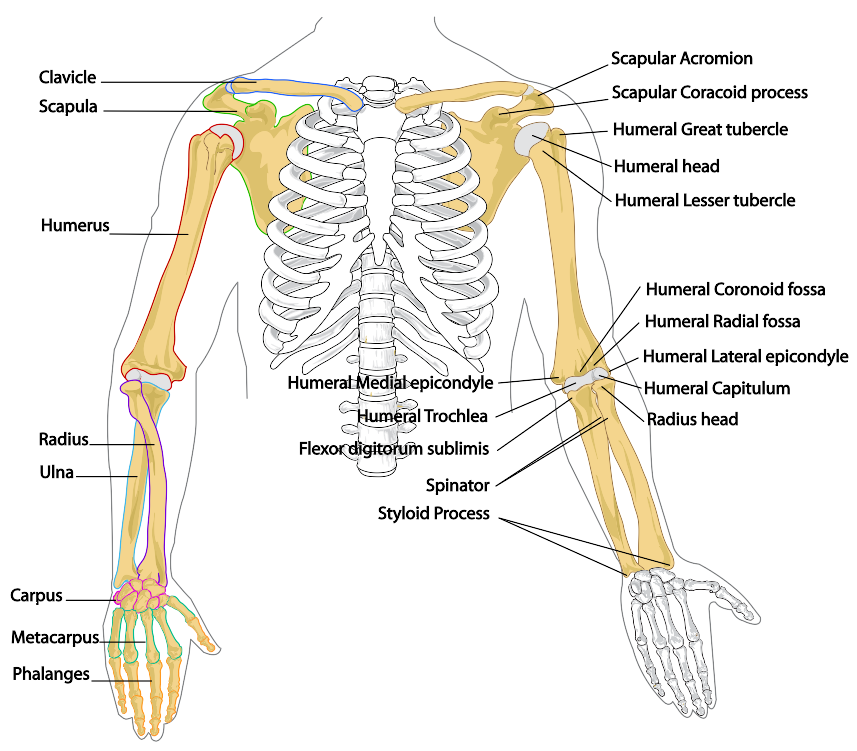
\includegraphics[width=.80\linewidth]{fig/Human_arm_bones_diagram}
\end{center}

\subsection{Myologie}

\begin{center}
        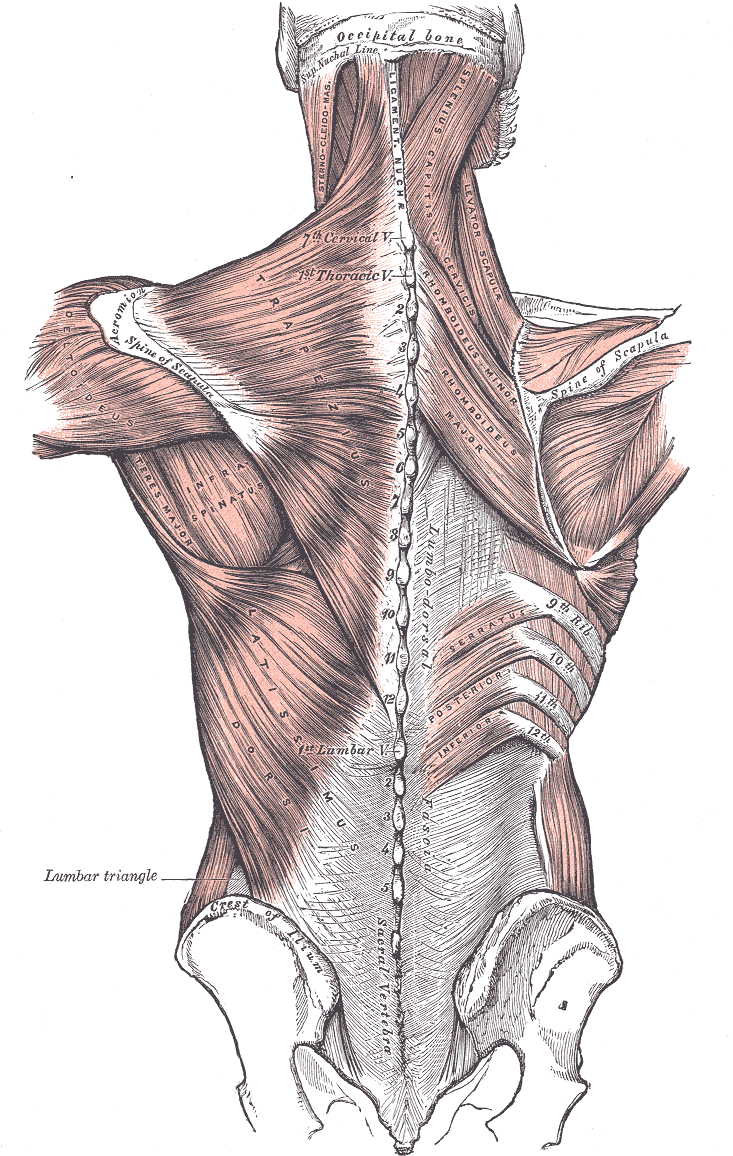
\includegraphics[width=.80\linewidth]{fig/Gray409}
\end{center}

\begin{center}
        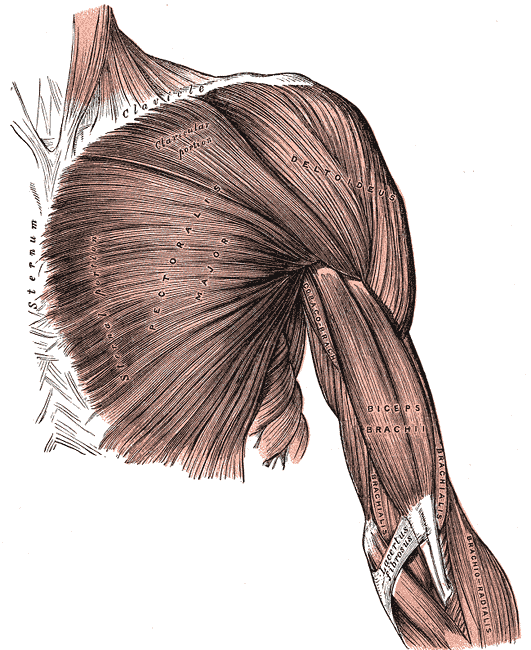
\includegraphics[width=.80\linewidth]{fig/Gray410}
\end{center}

\begin{center}
        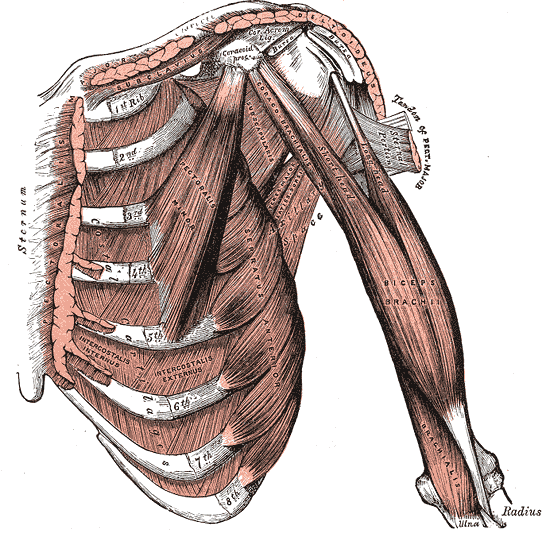
\includegraphics[width=.80\linewidth]{fig/Gray411}
\end{center}

\begin{center}
        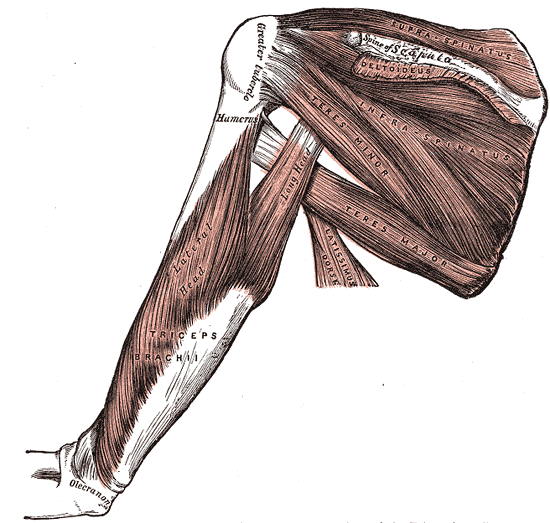
\includegraphics[width=.80\linewidth]{fig/Gray412}
\end{center}

\begin{center}
        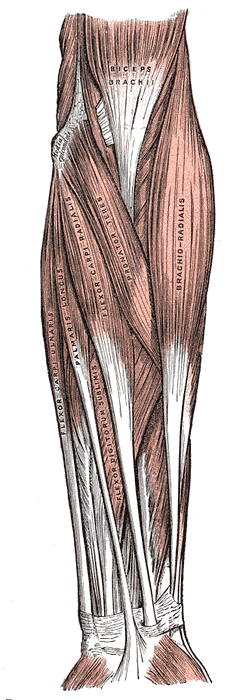
\includegraphics[width=.40\linewidth]{fig/Gray414}
\end{center}

\begin{center}
        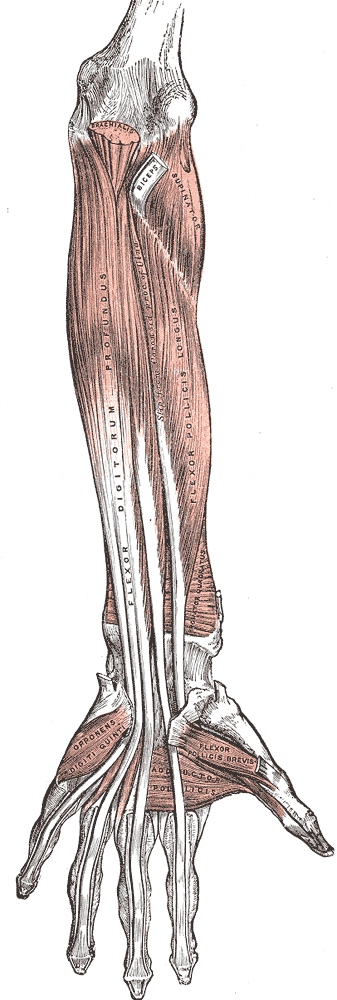
\includegraphics[width=.40\linewidth]{fig/Gray415}
\end{center}

\begin{center}
        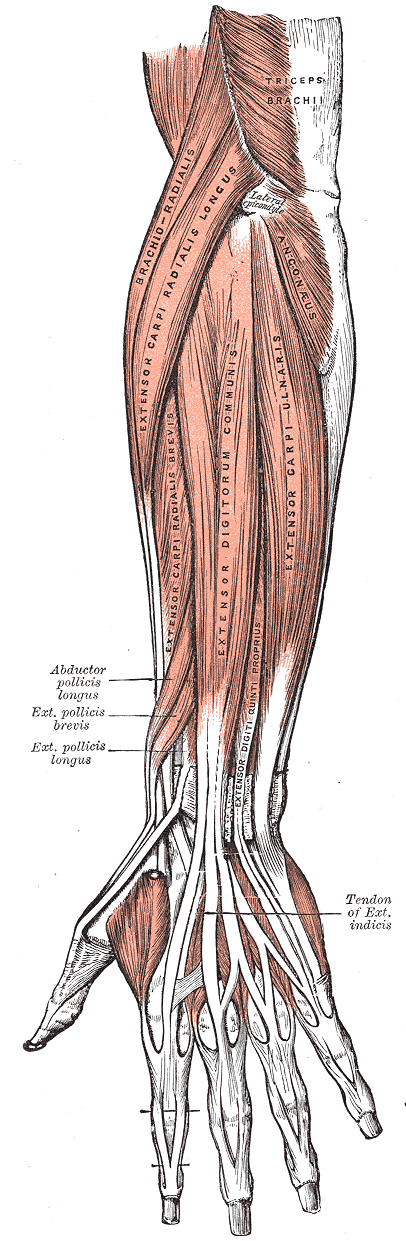
\includegraphics[width=.40\linewidth]{fig/Gray418}
\end{center}

\begin{center}
        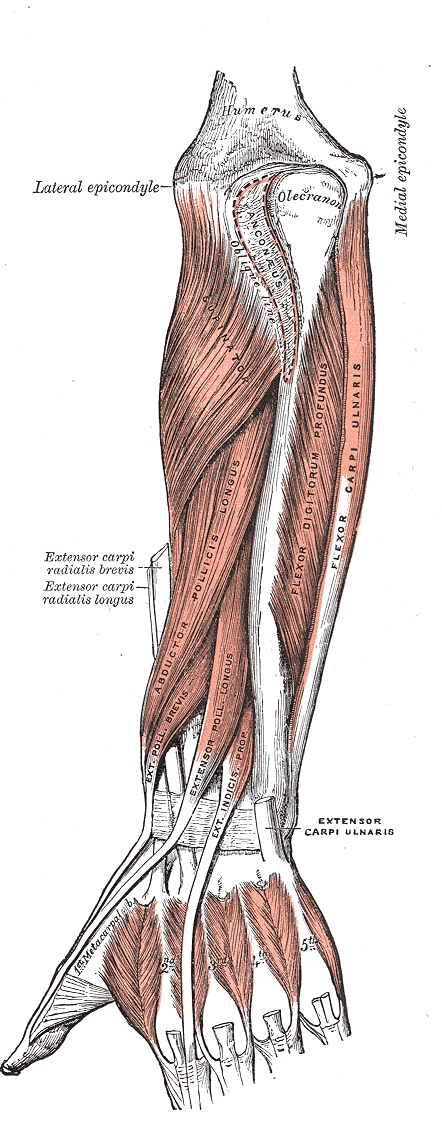
\includegraphics[width=.40\linewidth]{fig/Gray419}
\end{center}

\paragraph{}
Muscles de l'épaule
\begin{itemize}
    \item Fléchisseur
    \begin{itemize}
        \item 
    \end{itemize}
    \item Extenseur
    \begin{itemize}
        \item 
    \end{itemize}

    \item Muscle deltoïde (deltoid)
    \item Muscle sus-épineux ()
    \item Muscle sous-épineux ()
    \item Muscle petit rond ()
    \item 
    \item 
\end{itemize}

\paragraph{}
Muscles du coude
\begin{itemize}
    \item Fléchisseur
    \begin{itemize}
        \item 
    \end{itemize}
    \item Extenseur
    \begin{itemize}
        \item 
    \end{itemize}

    \item Muscle brachial antérieur ()
    \item Muscle long supinateur ()
%    \item in front, the Brachialis
%    \item in front, the Brachioradialis
%    \item behind, the Triceps brachii
%    \item behind, the Anconæus
%    \item laterally, the Supinator
%    \item laterally, the common tendon of origin of the Extensor muscles
%    \item medially, the common tendon of origin of the Flexor muscles
%    \item medially, the Flexor carpi ulnaris
    \item 
    \item 
\end{itemize}

\paragraph{}
Muscles bi-articulaire
\begin{itemize}
    \item Fléchisseur
    \begin{itemize}
        \item Muscle biceps brachial (Biceps brachii)
    \end{itemize}
    \item Extenseur
    \begin{itemize}
        \item Muscle triceps brachial (Triceps brachii)
    \end{itemize}
\end{itemize}

\subsection{Arthrologie}

\begin{itemize}
    \item 
    \item 
    \item 
    \item 
    \item 
    \item 
    \item 
    \item 
\end{itemize}


%%%%%%%%%%%%%%%%%%%%%%%%%%%%%%%%%%%%%%%%%%%%%%%%%%%%%%%%%%%%%%%%%%%%%%%%%%%%%%%%

%\chapter*{Bibliographie}

%\cite{clef_de_référence}

\bibliographystyle{plain}
\bibliography{article}

\end{document}
